\documentclass[10pt]{article}
\usepackage[letterpaper,margin=0.82in]{geometry}
\usepackage{amsmath,amssymb,amsthm,mathtools}
\usepackage{microtype}
\usepackage{enumitem}
\usepackage{xcolor}
\usepackage{tikz}
\usetikzlibrary{arrows.meta,positioning,fit,calc}
\usepackage[hidelinks]{hyperref}

\definecolor{proved}{HTML}{287A4B}
\definecolor{finite}{HTML}{9B6A00}
\definecolor{open}{HTML}{B3261E}
\definecolor{measured}{HTML}{4A4FA8}
\definecolor{conjc}{HTML}{7A3E8F}
\definecolor{navy}{HTML}{34517D}
\definecolor{paperblue}{HTML}{F3F6FB}

\theoremstyle{plain}
\newtheorem{theorem}{Theorem}[section]
\newtheorem{proposition}[theorem]{Proposition}
\newtheorem{lemma}[theorem]{Lemma}
\newtheorem{corollary}[theorem]{Corollary}
\theoremstyle{definition}
\newtheorem{remark}[theorem]{Remark}
\newtheorem{question}[theorem]{Question}
\newtheorem*{conjecturenamed}{Conjecture (Kaser--Lemire)}

\newcommand{\F}{\mathbb F}
\newcommand{\Z}{\mathbb Z}
\newcommand{\Q}{\mathbb Q}
\newcommand{\E}{\mathcal E}
\newcommand{\Lam}{\Lambda}
\newcommand{\ceil}[1]{\left\lceil #1\right\rceil}
\newcommand{\flr}[1]{\left\lfloor #1\right\rfloor}
\newcommand{\Prim}{\mathrm{Prim}}
\newcommand{\Luniv}{L_{\mathrm{univ}}}
\newcommand{\Ggeom}{G_{\mathrm{geom}}}
\newcommand{\Tr}{\mathrm{Tr}}
\newcommand{\GR}{\mathrm{GR}}
\newcommand{\imax}{i_{\max}}
\newcommand{\kmin}{k_{\min}}

\newcommand{\proved}{\textcolor{proved}{\textsf{\textbf{\footnotesize PROVED}}}}
\newcommand{\finite}{\textcolor{finite}{\textsf{\textbf{\footnotesize FINITE}}}}
\newcommand{\measuredst}{\textcolor{measured}{\textsf{\textbf{\footnotesize MEASURED}}}}
\newcommand{\openstatus}{\textcolor{open}{\textsf{\textbf{\footnotesize OPEN}}}}
\newcommand{\conj}{\textcolor{conjc}{\textsf{\textbf{\footnotesize CONJECTURED}}}}

\setlist{nosep,leftmargin=1.5em}
\setlength{\parskip}{1.6pt}
\setlength{\abovedisplayskip}{4pt}
\setlength{\belowdisplayskip}{4pt}
\setlength{\abovedisplayshortskip}{2pt}
\setlength{\belowdisplayshortskip}{2pt}
\setlength{\textfloatsep}{7pt}

\title{\vspace{-2.2em}Half-degree irreducibles over $\F_2$:\\
barriers, negative results, and what to try next}
\author{Michael Bommarito}
\date{23 August 2026}

\begin{document}
\maketitle
\vspace{-1.2em}

\begin{center}
\fcolorbox{open}{open!5}{\parbox{0.93\linewidth}{\centering
\textbf{Status.} \emph{Nothing in this document proves the Kaser--Lemire
conjecture.} Several of the results recorded here are textbook theorems applied
to new data, and they are labelled as such. The purpose is to say precisely
what has been tried, what is provably blocked, and what a specialist might
still attack.}}
\end{center}

\begin{abstract}
For every $n$, is there a monic irreducible $f\in\F_2[x]$ of degree $n$ with
$\deg(f-x^n)\le\flr{n/2}$? The question is Lemire's (MathOverflow, 2011), and
Kaser and Lemire published it as a conjecture in 2014 with a
Barrett-reduction motivation. Reversing $f$ turns it into Legendre's conjecture
for $\F_2[t]$: a prime in the interval of length $2\sqrt X$ around $X=2^n$.
The Riemann hypothesis is a theorem in this setting (Weil), and it is
short of the conjecture by exactly one logarithm. This document is the
record of a systematic attack on that logarithm. We collect what is
unconditionally proved (an almost-all theorem with a sharp constant; an
infinite family for every in-window seed; the exact sieve output of the
window; certified witnesses to $n=3000$), and then six barriers, each
stated as a proposition with proof and exact scope, that between them
eliminate moduli-only Fourier arguments, group actions, the known
irreducibility-preserving construction toolbox, all lower-bound sieves at
the window's own level of distribution, Betti-number bounds on Katz's
parameter space, and the one available fixed-$q$ \emph{disproof} template.
We then re-pose the surviving geometric question --- a
degree/weight statement for the Adams twist of Katz's universal sheaf on
$\Prim_j$ --- and report exact $L$-function computations that make it
look alive rather than dead, together with the two named open statements
it reduces to. A short marked section records the working method,
including five occasions on which our own claims were wrong.
\end{abstract}

\tableofcontents

\section{Introduction}

\subsection{The conjecture and where it comes from}

Write $W_n=\{x^n+g\ :\ g\in\F_2[x],\ \deg g\le\flr{n/2}\}$ for the
\emph{half-degree window} at degree $n$; $|W_n|=2^{\flr{n/2}+1}$.

\begin{conjecturenamed}
For every $n\ge1$ the window $W_n$ contains a monic irreducible polynomial;
equivalently, there is a monic irreducible $f\in\F_2[x]$ of degree $n$ with
$\deg(f-x^n)\le\flr{n/2}$.
\end{conjecturenamed}

The question was posed publicly by Daniel Lemire on MathOverflow on 23 November
2011, under the title ``Can we always find such an irreducible polynomial of
degree $n$ where $\mathrm{degree}(p(x)-x^n)\le n/2$?''~\cite{MO81717}. It
appears as a conjecture in print in Kaser and Lemire, \emph{Strongly universal
string hashing is fast}~\cite{KL}, in the section ``GF Multilinear'': they
verify it for $L\in\{1,\dots,400\}$ against Arndt's table~\cite{Arndt} and
conjecture it in general. The motivation is computational. In a string-hashing
kernel one reduces a product modulo an irreducible $f$ of degree $n$ over
$\F_2$; Barrett reduction is cheapest when the non-leading part of $f$ is
confined to the bottom half of the coefficient range, because then a single
carry-less multiplication by the precomputed reciprocal suffices and the
correction step does not overflow. So the conjecture is exactly the assertion
that this optimization is always available.

The 2011 thread already contains most of the mathematical landscape.
Elkies and Zaimi both state the expected truth --- that the minimal
\emph{subdegree} $\deg(f-x^n)$ should be $O(\log n)$, not $n/2$ --- and Arndt's
table bears this out: the minimal subdegree is at most $10$ for every
$n\le400$. Ellenberg gives the framing that organizes everything below: this is
Legendre's conjecture for $\F_2[t]$, and Cram\'er's heuristic under RH buys
intervals of length about $\sqrt X\log X$, i.e.\ subdegree $n/2+\log n$, one
logarithm on the wrong side. Voloch notes that Cohen's prescribed-coefficient
criterion likewise stops at $m<n/2+O(\log n)$. And Emil Je\v{r}\'abek's comment
gives the infinite family $x^{2\cdot3^k}+x^{3^k}+1=\Phi_{3^{k+1}}$, which is an
exercise in Lidl--Niederreiter, so that the degrees $n=2\cdot3^k$ have been
settled since 2011.

\subsection{The one-line reason it is hard}

Reversing $f\mapsto f^*(T)=T^{\deg f}f(1/T)$ converts the window condition into
a congruence (Section~\ref{sec:setting}): $W_n$ contains an irreducible if and
only if there is a prime $P\in\F_2[T]$ of degree $n$ with
$P\equiv1\pmod{T^{\ceil{n/2}}}$. Thus the conjecture is
\emph{Legendre's conjecture for $\F_2[t]$}: a prime in a short interval of
length $2^{\ceil{n/2}}$, i.e.\ between $\sqrt X$ and $2\sqrt X$ where
$X=2^n$. Equivalently it is Linnik's problem with exponent exactly $2$, for
the residue $1$ and the prime-power modulus $T^{\ceil{n/2}}$.

Over $\Z$ this is hopeless because RH is unavailable. Here RH \emph{is}
available: it is Weil's theorem, and it gives, for every Hayes character $\chi$
of conductor $j$,
\[
 |S_n(\chi)|\ :=\ \Bigl|\sum_{\deg F=n}\Lam(F)\chi(\langle F\rangle_j)\Bigr|
 \ \le\ (j-1)\,2^{n/2}.
\]
Summing this over the $2^{\ell}$ characters, with $\ell=\ceil{n/2}-1$, gives a
main term $2^{n-\ell}$ against an error $\sum_j 2^{j-1}(j-1)2^{n/2}\approx
\ell2^{\ell}2^{n/2}$, and the two are the same size up to the factor $\ell$.
That factor is the whole problem. The classical statement of the same
phenomenon: the top $n/2-\log_2 n$ coefficients of an irreducible are
prescribable unconditionally (Hayes plus Weil, in the sharp form of
Hsu~\cite{Hsu} $=$ Cohen~\cite{Cohen}), and Kaser--Lemire asks for
$\ceil{n/2}-1$ of them. \textbf{The conjecture is exactly the removal of the
$\log$ that RH leaves behind.} It is not a power gap; it is the classical
square-root barrier, transplanted to a setting where the square-root barrier
is a theorem rather than a hypothesis.

\subsection{What this document is, and is not}

It is a companion to the three-page roadmap note~\cite{roadmap}, which states
the reduction chain and the single open estimate, and to the almost-all
note~\cite{almostall}. Where those are compressed, this one is expansive: it
records the negative results, which are the part of the work that is most
likely to save a reader time.

Three things it is not. It is not a proof, and it does not contain a plausible
sketch of one. It is not a survey of the function-field literature: papers are
cited only where they bear on this window at $q=2$, and the fixed-$q$,
growing-conductor regime is essentially untouched in print. And it is not a
claim of novelty for most of what it proves: the almost-all theorem is
Parseval$+$Weil$+$Chebyshev, the infinite family is
Lidl--Niederreiter~\cite{LN} Theorem 3.35 applied to a certified seed ledger,
and the sieve output is Jurkat--Richert applied to a sequence with exact
divisor data. Each such statement is labelled where it appears.

\paragraph{Status tags.} Every substantive claim below carries one of five
tags, and the distinctions are enforced rather than decorative:
\begin{itemize}
\item \proved{} --- a theorem, with a proof here or an exact citation.
\item \finite{} --- machine-checked finite evidence: an exact computation over
  a stated finite range, re-verified by an independent engine and gated by a
  checker that exits nonzero on failure.
\item \measuredst{} --- a measurement or a heuristic model fit; a number, not a
  theorem, and not a proof of the asymptotic it suggests.
\item \openstatus{} --- open, with the precise statement given.
\item \conj{} --- conjectured here or in the literature, with the source.
\end{itemize}
Internal sources are cited by lane note number (``note 13''); these are the
research notes in \texttt{docs/\allowbreak research/\allowbreak 10-cas/\allowbreak lemire-signed-trace/} of the
repository~\cite{ledger}, together with the checkers in
\texttt{scripts/lemire-signed-trace/}. Where a claim is machine-checked, the
script that checks it is named.


\section{Setting and the reduction}\label{sec:setting}

This section is compressed; the full chain, with the endpoint bookkeeping, is
in the roadmap note~\cite{roadmap}. Everything in it is \proved.

\paragraph{The ray class group.} For $j\ge0$ put
\[
 \E_j\ =\ (1+x\F_2[x])/(x^{j+1})\ =\ \bigl(\F_2[x]/x^{j+1}\bigr)^{\times},
 \qquad |\E_j|=2^{j},
\]
and for monic $F$ let $\langle F\rangle_j=x^{\deg F}F(x^{-1})\bmod x^{j+1}$.
With $\ell=\ceil{n/2}-1$, the window condition $\deg(f-x^n)\le\flr{n/2}$ is
exactly $\langle f\rangle_\ell=1$. So Kaser--Lemire asks for a prime of degree
$n$ in the \emph{identity ray class} of $\E_\ell$.

By Artin--Hasse, $\E_j$ is the truncated big Witt ring of $\F_2$ and splits
(Katz~\cite{Katz13}, Lemma 2.2) as
$\E_j\cong\prod_{k\ \mathrm{odd}\le j}\Z/2^{e_k}$ with
$e_k=\flr{\log_2(j/k)}+1$ and $\sum_k e_k=j$. Under this splitting the class of
$\alpha\in\F_{2^n}$ is the vector of Galois-ring traces
$\Tr_{\GR(2^{e_k},n)}(\tilde\alpha^{\,k})\bmod 2^{e_k}$ of the Teichm\"uller
lift, so the identity class is the locus where \emph{all odd-power traces
vanish to prescribed dyadic precisions}. This is the description that makes
the class genuinely distinguished, and every barrier in Section~\ref{sec:barriers}
is in the end a statement about that.

\paragraph{Hayes characters and the Weil bound.} The characters of $\E_j$ are
the even Hayes characters modulo $x^{j+1}$~\cite{Hayes}. For $\chi$ of exact
conductor $j$, $L(\chi,T)=\prod_{i\le j-1}(1-\alpha_i T)$ is a polynomial of
degree $j-1$, pure of weight one ($|\alpha_i|=\sqrt2$) by Weil~\cite{Weil}, and
\[
 S_n(\chi)=\sum_{\deg F=n}\Lam(F)\chi(\langle F\rangle_j)=-\sum_i\alpha_i^{\,n},
 \qquad |S_n(\chi)|\le(j-1)2^{n/2}.
\]
Conductor $1$ gives $L=1$, hence $S_n=0$. Exactly $2^{j-1}$ characters have
exact conductor $j$.

\paragraph{The telescope and (REL).} Write
$N_j(g)=\sum_{\deg F=n,\ \langle F\rangle_j=g}\Lam(F)$. Binary splitting of the
two-element fibres of $\E_j\to\E_{j-1}$ gives the Haar telescope
$2^{\ell}N_\ell(e)=2^n+\sum_{j\le\ell}\varepsilon_j(e)2^{j-1}H_j(b_j(e))$ with
$H_j$ the difference of the two child populations. Put
$c=\ceil{\log_2\ell}$, $a=\ell-c-1$,
\[
 C_{\ell,n}=\sum_{j=a}^{\ell}2^{j-1}H_j(1),
 \qquad
 B_{\ell,n}=2^{2\ell}-2^{\ceil{n/2}}\sum_{1\le j<a}(j-1)2^{j-1}\ >\ 0 .
\]
Summing the large conductors \emph{before} taking absolute values telescopes
them, and the proper-power count at both endpoints reduces the conjecture to
\[
 \textrm{(REL)}\qquad C_{\ell,n}\ >\ -B_{\ell,n}.
\]

\paragraph{Order layers and (HWO).} Let $2^s\E_j$ be the $2^s$-power subgroup,
$P_{j,s}=\sum_{g\in2^s\E_j}N_j(g)$, $h_{j,s}=2^{\,j-\flr{j/2^s}}$, and
\[
 T_{j,s}(n)\ =\ h_{j,s}P_{j,s}-h_{j,s-1}P_{j,s-1}-h_{j-1,s}P_{j-1,s}
 +h_{j-1,s-1}P_{j-1,s-1}
\]
the sum of $S_n(\chi)$ over the $\#X_{j,s}$ characters of exact conductor $j$
and exact order $2^s$. With $Q$ the largest power of two with $3Q\ceil{\log_2\ell}\le\ell$,
the Weil bound pays for every layer of order at most $Q$, and what remains is
\[
 \textrm{(HWO)}\qquad
 4\ell\,|T_{j,s}(n)|\ \le\ \#X_{j,s}\,(j-1)\,2^{\ceil{n/2}}
 \qquad(a\le j\le\ell,\ 2^s>Q),
\]
i.e.\ a factor $4\ell$ of saving over Weil for the \emph{signed} sum over a
complete layer, uniformly in $\ell$. \textbf{(HWO) $\Rightarrow$ (REL)
$\Rightarrow$ Kaser--Lemire, and this implication is proved} (note 01;
endpoint ledger replayed for $200\le\ell\le1024$). A necessary
conductor/order case split makes (HWO) equivalent to a sparse-discrepancy
statement: with $d_s=\flr{(j-1)/2^s}$, $\Delta_{j,s}=2P_{j,s}-P_{j-1,s}$ and
$R=2^{d_{s-1}-d_s}$,
\[
 \textrm{(NSD)}\ \ 4\ell|R\Delta_{j,s}-\Delta_{j,s-1}|\le(R-1)(j-1)2^{\ceil{n/2}}
 \quad\text{when } 2^{s-1}\nmid j,
\]
\[
 \textrm{(RSD)}\ \ 4\ell|\Delta_{j,s}|\le(j-1)2^{\ceil{n/2}}
 \quad\text{when } 2^{s-1}\mid j,\ 2^s\nmid j .
\]
The resonant case is not a small-scale artefact: at $j=\ell=200$ the order
$2^s=16$ is high and $8\mid200$, $16\nmid200$.

\paragraph{The cylinder form (CYL).} Let $K=\ker(\E_\ell\to\E_{a-1})$, of order
$2^{\ell-a+1}=2^{c+2}$, so that
\begin{equation}\label{eq:ksize}
 4\ell\ \le\ |K|\ <\ 8\ell .
\end{equation}
For $\psi\in\widehat K$ put $A_\psi=\sum_{g\in K}N(g)\psi(g)$, the prime mass of
the cylinder $\{x^n+g:\deg g\le n-a\}$ twisted by a sign pattern of the
$c+2$ coefficients of $x^{n-a},\dots,x^{n-\ell}$. Fourier inversion on $K$ gives
\[
 \textrm{(CYL)}\qquad |A_\psi|<2^{\ell-1}\ \text{ for every }\psi\ne1
 \qquad\Longrightarrow\qquad \textrm{(REL)} .
\]
(CYL) is the weakest sufficient statement currently known, and it is the
ledger's open fact \texttt{F:gf2-\allowbreak lemire-\allowbreak cylinder-\allowbreak twist-\allowbreak sup-bound}. Weil gives
only $|A_\psi|\le(\ell-1)2^{\ceil{n/2}}$, a factor $4(\ell-1)$ short.

\paragraph{The reversal duality, with the index.}
Keating--Rudnick's involution~\cite{KR} ($f\mapsto f^*$, $\Lam(f^*)=\Lam(f)$
when $f(0)\ne0$) gives the bijection
\[
 \{f\ \text{monic irred.},\ \deg f=n,\ \deg(f-T^n)\le\flr{n/2}\}
 \ \longleftrightarrow\
 \{P\ \text{monic irred.},\ \deg P=n,\ P\equiv1\!\!\pmod{T^{\,r}}\},
\]
with
\[
 \boxed{\ r\ =\ n-\flr{n/2}\ =\ \ceil{n/2}\ =\ \ell+1\ }
\]
\proved{} (note 16; \texttt{lemire\_largeq.py}, verified on 89 pairs $(q,n)$
and 24{,}090 polynomials, $q\in\{2,3,4,5,7,8,9\}$, $n\le24$).

\begin{remark}[the off-by-one is not cosmetic]
The naive index $\flr{n/2}+1$ agrees with $\ceil{n/2}$ at odd $n$ and is
\emph{one too large} at even $n$. This changes the level of distribution
required from exactly $1/2$ to $1/2+1/n$, hence whether $\omega=1/2$ is
admissible at all; and it can change the answer. Over $\F_3$ at $n=4$ there
are $6$ in-window irreducibles, $2$ of them with $f(0)=1$, matching the
progression count at $r=2$; at $r=3$ the progression is \emph{empty}. An
argument run at the wrong index would have concluded that no in-window
irreducible of degree $4$ exists over $\F_3$, which is false. (Note 16; the
checker's mutation control changes $r$ and kills exactly the three duality
checks.)
\end{remark}

\begin{figure}[t]
\centering
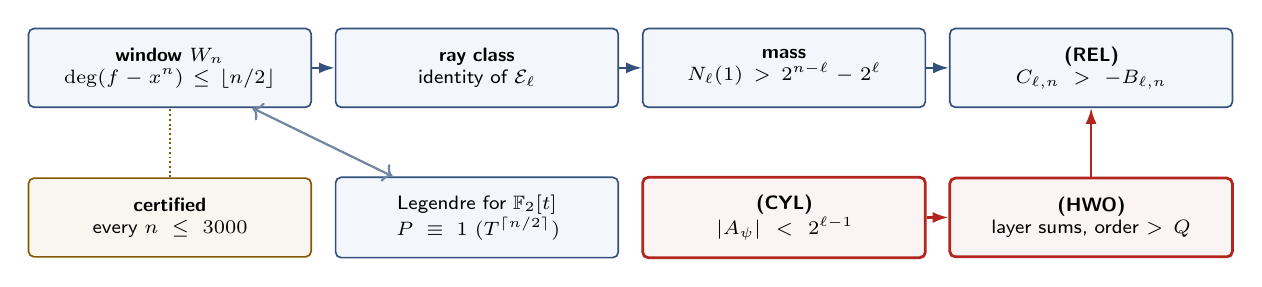
\begin{tikzpicture}[
  x=1cm,y=1cm,
  box/.style={draw=navy,fill=paperblue,rounded corners=2pt,line width=.6pt,
    text width=3.15cm,align=center,inner sep=2.2mm,font=\sffamily\scriptsize,
    minimum height=1.0cm},
  redbox/.style={box,draw=open,fill=open!5,line width=1.0pt},
  goldbox/.style={box,draw=finite!85!black,fill=finite!6},
  arr/.style={-{Latex[length=2mm,width=1.4mm]},line width=.8pt,draw=navy}
]
\node[box] (w) at (0,0) {\textbf{window} $W_n$\\ $\deg(f-x^n)\le\flr{n/2}$};
\node[box] (r) at (3.9,0) {\textbf{ray class}\\ identity of $\E_\ell$};
\node[box] (m) at (7.8,0) {\textbf{mass}\\ $N_\ell(1)>2^{n-\ell}-2^\ell$};
\node[box] (rel) at (11.7,0) {\textbf{(REL)}\\ $C_{\ell,n}>-B_{\ell,n}$};
\node[redbox] (hwo) at (11.7,-1.9) {\textbf{(HWO)}\\ layer sums, order $>Q$};
\node[redbox] (cyl) at (7.8,-1.9) {\textbf{(CYL)}\\ $|A_\psi|<2^{\ell-1}$};
\node[goldbox] (cert) at (0,-1.9) {\textbf{certified}\\ every $n\le3000$};
\node[box] (leg) at (3.9,-1.9) {Legendre for $\F_2[t]$\\ $P\equiv1\ (T^{\ceil{n/2}})$};
\draw[arr] (w)--(r); \draw[arr] (r)--(m); \draw[arr] (m)--(rel);
\draw[arr,draw=open] (hwo)--(rel);
\draw[arr,draw=open] (cyl)--(hwo);
\draw[arr,<->,draw=navy!70] (w)--(leg);
\draw[draw=finite!85!black,densely dotted,line width=.7pt] (cert)--(w);
\end{tikzpicture}
\caption{The reduction chain. Blue arrows are proved implications; the two red
boxes are the open sufficient statements, either of which closes the chain.
The gold box is the finite verification, which is insurance and not evidence
for the open step. The double arrow records that the window question
\emph{is} Legendre's conjecture for $\F_2[t]$, so no argument blind to the
centre of the interval can separate them (Section~\ref{sec:barriers}, Barrier IV).}
\label{fig:chain}
\end{figure}
\section{What is proved}\label{sec:proved}

\subsection{Certified witnesses to \texorpdfstring{$n=3000$}{n = 3000}}

\begin{proposition}[\finite]\label{prop:cert}
For every $n\le3000$ the window $W_n$ contains an explicit irreducible
polynomial, doubly certified.
\end{proposition}

For $401\le n\le3000$ each witness is sparse, $x^n+\sum x^{e_i}+1$ with every
$e_i\le\flr{n/2}$, and carries a Frobenius/B\'ezout irreducibility certificate
that is re-verified by an independent checker: $2600$ of $2600$ pass, $1334$
trinomials and $1266$ pentanomials. The replayable table (degree, tail
exponents, SHA-256 of the artifact, check status) is
\texttt{data/witnesses-401-3000-sha256.tsv}. A third, independent flint-based
search with pure-Python Rabin re-verification agrees on existence for every
degree in $401..842$, producing identical trinomial witnesses (note 02
\S6; \texttt{lemire\_witness\_search.py}).

Two honest remarks. First, powers of two need denser witnesses: Swan's theorem
forbids an irreducible trinomial of any degree divisible by $8$, which is why
roughly half the table is pentanomials. Second, and more important, this is
\emph{insurance, not evidence}: combined with the reduction, the chain is
complete for $n\le3000$ and for all $n$ once (HWO) or (CYL) holds for
$\ell\ge1500$. It says nothing about the open estimate.

\subsection{The almost-all theorem}

\begin{theorem}[\proved; note 05, \texttt{lemire\_almostall.py}]\label{thm:aa}
Let $\ell\ge1$, $n\in\{2\ell+1,2\ell+2\}$, $0<t\le1$, and put
$\varepsilon(\ell)=(\ell^2-4\ell+6)-6\cdot2^{-\ell}$ and
$\kappa_n=2^{2\ceil{n/2}-n}\in\{1,2\}$. Then
\[
 \#\bigl\{g\in\E_\ell\ :\ |N_\ell(g)-2^{n-\ell}|\ge t\,2^{n-\ell}\bigr\}
 \ \le\ \kappa_n\,2^{2\ell-n}\,\varepsilon(\ell)/t^2 .
\]
Consequently, for $\ell\ge5$, the number of top-half patterns
$h\in\F_2^{\ell}$ carried by \emph{no} irreducible of degree $n$ is at most
$4(\ell^2-4\ell+6)<4\ell^2$ for odd $n$ and at most $\ell^2-4\ell+6<\ell^2$ for
even $n$; so all but a fraction $<4\ell^2 2^{-\ell}$ of the $2^{\ell}$ patterns
are realized.
\end{theorem}

\begin{proof}[Proof sketch]
Parseval on $\E_\ell$ turns $\sum_g(N_\ell(g)-2^{n-\ell})^2$ into
$2^{-\ell}\sum_{\chi\ne1}|S_n(\chi)|^2$; Weil and the conductor count give
$\sum_{\chi\ne1}|S_n|^2\le2^{2\ceil{n/2}}\sum_{j=1}^{\ell}2^{j-1}(j-1)^2
=2^{2\ceil{n/2}}A(\ell)$ with
$A(\ell)=\sum_{i=1}^{\ell-1}i^2 2^i=2^{\ell}(\ell^2-4\ell+6)-6$ (induction);
Chebyshev finishes. The irreducible count follows after a Markov bound on the
proper-power mass, which is empty for odd $n$ and has at most one exceptional
class for even $n$.
\end{proof}

\paragraph{Honest scope.} This is Parseval $+$ Weil $+$ Chebyshev: the
function-field Barban--Davenport--Halberstam second moment, unconditional here
only because RH is Weil's theorem. The method is standard; the endpoint
statement with explicit constants at fixed $q=2$ we did not find in print, and
it should be treated as folklore made explicit, not as new. Hayes~\cite{Hayes}
and Hsu~\cite{Hsu} give \emph{pointwise} asymptotics for every class while
$\ell\le n/2-\log_2\ell-O(1)$ --- stronger in that range, failing exactly at the
last $\log_2\ell$ coefficients, which is the entire gap.

\paragraph{What it measures.} The exceptional set is \emph{empty} at every size
computed ($\ell\le24$), while the theorem allows $10\%$ of classes at
$\ell=12$; the worst class is $0.3$--$13\%$ off the mean, and
$\min_g N_\ell(g)/\mathrm{mean}=0.9971$ at $(\ell,n)=(24,50)$ (\finite). The
observed second moment is at its Sato--Tate value to three digits from
$\ell=16$ on, so Weil is lossy here by exactly the expected factor $\sim\ell$
(\measuredst). Per conductor, the second moment \emph{saturates} the sharp Weil
bound at $j=2$ (ratio $1.00000$ at every endpoint) and sits at
$\mathrm{rms}|S|/((j-1)2^{n/2})=1/\sqrt{j-1}$ to four digits at $j=24$: Weil is
attained at the stabilizer boundary and $\sqrt{j-1}$-lossy above it.

\paragraph{The residual.} Kaser--Lemire is exactly the statement that
\emph{one named pattern}, $h=0$, is not exceptional. Theorem~\ref{thm:aa}
cannot address it, and not for want of constants: its three inputs are
invariant under permutations of $\E_\ell$. Barrier I
(\S\ref{sec:bar1}) makes that precise.

\subsection{The monomial-composition family}

\begin{theorem}[\proved; note 08 Theorem A, \texttt{lemire\_composition\_family.py}]
\label{thm:family}
Let $f\in\F_2[x]$ be irreducible of degree $m$ with $f(0)\ne0$, of order
$e=\mathrm{ord}(f)$, and suppose $f$ is in-window, i.e.\
$\deg(f-x^m)\le\flr{m/2}$. Let $t\ge2$ satisfy
\begin{enumerate}[label=(\roman*)]
\item $\mathrm{rad}(t)\mid e$: every prime divisor of $t$ divides $e$; and
\item $\gcd(t,(2^m-1)/e)=1$.
\end{enumerate}
Then $f(x^t)$ is an in-window irreducible of degree $mt$ and order $et$. Hence
Kaser--Lemire holds at $n=mt$.
\end{theorem}

\begin{proof}
Irreducibility is Lidl--Niederreiter~\cite{LN} Theorem 3.35 (stated there in
exhaustive form; the single-polynomial ``iff'' form is Handbook of Finite
Fields~\cite{Handbook} Thm.\ 3.2.5, after Menezes et al.). At $q=2$ the fourth
hypothesis of the book's statement ($q^m\equiv1\bmod4$ when $4\mid t$) is
vacuous, because $e\mid2^m-1$ is odd and (i) already forces $t$ odd. The window
is the one-line observation: monomial substitution scales tail and degree by
the \emph{same} factor,
\[
 f(x^t)-x^{mt}=(f-x^m)(x^t),
 \qquad
 \deg\bigl(f(x^t)-x^{mt}\bigr)=t\deg(f-x^m)\le t\flr{m/2}\le\flr{mt/2},
\]
the last inequality for every $t\ge1$ (equality when $m$ is even; for $m$ odd it
reads $t(m-1)/2\le(mt-1)/2$). Machine-checked for all $m<200$ and all odd
$t<200$.
\end{proof}

\paragraph{Credit.} Nothing here is new mathematics. The irreducibility half is
a textbook criterion; the contribution is the observation that the window costs
nothing, so the criterion transports Kaser--Lemire from a seed degree to all
its admissible multiples. The $m=2$ case is the cyclotomic family
$\Phi_{3^{k+1}}=x^{2\cdot3^k}+x^{3^k}+1$, $n=2\cdot3^k$, which
Je\v{r}\'abek gave on MathOverflow in November 2011 --- the same thread in
which the conjecture was posed --- and which in one direction reproves the
classical trinomial fact that $x^{2k}+x^k+1$ is irreducible over $\mathrm{GF}(2)$
if and only if $k$ is a power of $3$ (Fredricksen--Wisniewski~\cite{FW};
see also Golomb--Lee~\cite{GolombLee}).

\paragraph{Operational criterion.} Hypotheses (i)--(ii) collapse to: for every
prime $p\mid t$, $v_p(e)=v_p(2^m-1)\ge1$, i.e.\ $p\mid2^m-1$ and
$x^{(2^m-1)/p}\ne1$ in $\F_2[x]/(f)$. This needs \emph{no} factorization of
$2^m-1$ --- one modular exponentiation per candidate prime --- and the candidate
primes are found from $\mathrm{ord}_p(2)\mid m$. Write $A(f)$ for the resulting
set of \emph{admissible primes}; Theorem~\ref{thm:family} applies to exactly
those $t$ all of whose prime factors lie in $A(f)$. If $f$ is primitive, $A(f)$
is the full set of prime divisors of $2^m-1$.

\begin{table}[t]
\centering\small
\begin{tabular}{llcll}
\hline
seed $f$ & $m$ & $e$ & $A(f)$ & degrees reached\\
\hline
$x^2+x+1$ & 2 & 3 & $\{3\}$ & $n=2\cdot3^k$\\
$x^3+x+1$ & 3 & 7 & $\{7\}$ & $n=3\cdot7^k$ \quad(\textbf{odd})\\
$x^4+x+1$ & 4 & 15 & $\{3,5\}$ & $n=4\cdot3^a5^b$\\
$x^5+x^2+1$ & 5 & 31 & $\{31\}$ & $n=5\cdot31^k$ \quad(\textbf{odd})\\
$x^6+x+1$ & 6 & 63 & $\{3,7\}$ & $n=6\cdot3^a7^b$\\
$x^8+x^4+x^3+x^2+1$ & 8 & 255 & $\{3,5,17\}$ & $n=8\cdot3^a5^b17^c$\\
$x^9+x^4+1$ & 9 & 511 & $\{7,73\}$ & $n=9\cdot7^a73^b$ \quad(\textbf{odd})\\
$x^{12}+x^6+x^4+x+1$ & 12 & 4095 & $\{3,5,7,13\}$ & $n=12\cdot3^a5^b7^c13^d$\\
\hline
\end{tabular}
\caption{Seeds and the degrees they reach (note 08). Explicit odd witnesses,
verified irreducible and in-window by two independent engines:
$x^{21}+x^7+1$, $x^{147}+x^{49}+1$, $x^{1029}+x^{343}+1$,
$x^{7203}+x^{2401}+1$ ($m=3$), and $x^{155}+x^{62}+1$ ($m=5$, $t=31$).}
\label{tab:seeds}
\end{table}

\begin{table}[t]
\centering\small
\begin{tabular}{lrrrr}
\hline
$N$ & $\#(S\cap[1,N])$ & $\#S/N$ & composites $\le N$ & fraction of composites\\
\hline
$10^2$ & 22 & 0.2200 & 74 & 0.297\\
$10^3$ & 243 & 0.2430 & 831 & 0.2924\\
$10^4$ & 2086 & 0.2086 & 8770 & 0.2379\\
$10^5$ & 8394 & 0.0839 & 90407 & 0.0929\\
\hline
\end{tabular}
\caption{Exact coverage of Theorem~\ref{thm:family} applied to a ledger of
certified in-window seeds of every degree $m\le3000$ (\finite;
\texttt{data/composition-coverage.txt}). The apparent health of the first three
rows and the drop in the fourth are both artefacts of the ledger, not
densities: see the discussion of (B4) in \S\ref{sec:bar3}.}
\label{tab:coverage}
\end{table}

\paragraph{Coverage and its honest reading.} Applied to a ledger $L$ of known
seeds --- here, one certified in-window irreducible for every $m\le3000$ plus
every in-window irreducible found by a bounded per-degree search --- the theorem
proves the conjecture on
$S(L,N)=\{mt\le N: m\in L,\ t\ge2,\ \mathrm{rad}(t)\subseteq A(f)\ \text{for one
seed }f\ \text{of degree }m\}$. Note the quantifier: the primes of a single $t$
must all be admissible for \emph{one} seed. Table~\ref{tab:coverage} gives the
exact counts; $411$ members are re-verified by a direct Rabin certificate on
$f(x^t)$ (degrees $6$ to $20000$) and $220$ of those a third time by
python-flint. The smallest composite \emph{not} in $S$ is $4$; the smallest odd
composite not in $S$ is $9$. No prime and no power of two is ever in $S$.
Asymptotically, $\max_f|A(f)|=16$ over this ledger (first attained at $m=360$),
so $\#S(L,N)=O((\log N)^{16})$ and the density is zero --- but the implied bound
evaluates to $6.5\times10^7$ at $N=10^5$, so it exceeds $N$ over the whole
computed range: \textbf{density zero here is proved asymptotically and not
observed}.

\paragraph{And the truth is far stronger.} Theorem~\ref{thm:family} produces
witnesses whose tail sits at exactly $t\deg(f-x^m)$, i.e.\ at the top of the
window, whereas the minimal subdegree in Arndt's table is $\le10$ for every
$n\le400$ and tracks $\sim\log_2 n$. The construction is nowhere near the
observed behaviour; the analytic ceiling ($n/2-\log_2 n$) matches it much better.

\subsection{What the sieve proves}\label{sec:sievepos}

Write $h=\flr{n/2}+1$, so $|W_n|=2^h$ and $\ell=n-h$. All of the following is
\proved{} (note 13), machine-checked by \texttt{lemire\_sieve\_face.py} with
six mutation controls, each shown to trip.

\begin{lemma}[exact Type I]\label{lem:typeI}
Let $d$ be monic of degree $k$, let $d^*=x^kd(1/x)$ and
$c=(d^*)^{-1}\bmod x^{\ell+1}$. Then
\[
 A_d:=\#\{F\in W_n: d\mid F\}=2^{\,h-k}\quad(0\le k\le h),
 \qquad
 A_d=\mathbf1[\deg c\le n-k]\quad(h<k\le n).
\]
In particular the remainder $r_d=A_d-|W_n|/|d|$ is \emph{identically zero} for
every monic $d$ of degree $\le h$, so $W_n$ has level of distribution
$D=|W_n|=2^h$ with no error term at all.
\end{lemma}

\begin{proof}
$F=dm$ with $m$ monic of degree $n-k$, and reversal is multiplicative:
$F^*=d^*m^*$. The window condition is $F^*\equiv1\bmod x^{\ell+1}$, i.e.\
$m^*\equiv(d^*)^{-1}\bmod x^{\ell+1}$. As $m$ runs over monics of degree $n-k$,
$m^*$ runs over all polynomials of degree $\le n-k$ with constant term $1$, so
$n-k$ free coefficients are prescribed in positions $1,\dots,\ell$; if
$k\le h$ then $h-k$ remain free.
\end{proof}

This is strictly better than the integer analogue, where $[x,x+\sqrt x]$ has
$|r_d|\le1$ and the level is $\sqrt x/\log x$. It is also \emph{best possible}.

\begin{corollary}[no level beyond $|W_n|$, not even on average]\label{cor:nolevel}
For $k>h$, $\sum_{\deg d=k}|r_d|=2(2^h-2^{2h-k})\to2|W_n|$. So there is no
Bombieri--Vinogradov-style averaged level past $2^h$ either: the total
remainder at any single level above $h$ is twice the size of the whole set.
\end{corollary}

\begin{corollary}[the sieve sees only ``an interval'']\label{cor:unif}
For \emph{every} monic $A_0$ of degree $n$, the interval
$I(A_0)=\{F:\deg(F-A_0)<h\}$ has $\#\{F\in I(A_0):d\mid F\}=2^{h-k}$ exactly,
for every monic $d$ of degree $k\le h$.
\end{corollary}

The sieve axioms hold with dimension $\kappa=1$; Mertens over $\F_q[t]$ is
exact ($\log(1/V(y))=\sum_{N\le y}1/N+R_y$ with $|R_y|\le4q^{-y/2}$, so
$V(y)=e^{-\gamma}/y\,(1+O(1/y))$ with no $q$-dependent constant), and the
Jurkat--Richert linear sieve~\cite{FI} applies with the remainder sum
identically zero. The sifting parameter at the prime level is
$s=h/(n/2)=1+2/n\to1$, which is the parity line.

\begin{theorem}[what the linear sieve gives]\label{thm:sieveout}
\mbox{}
\begin{enumerate}[label=(\alph*)]
\item ($P_4$) For every $\epsilon>0$ and $n\ge n_0(\epsilon)$, $W_n$ contains an
$F$ all of whose irreducible factors have degree $>(\tfrac14-\epsilon)n$; four
such factors would overflow the degree, so $\Omega(F)\le4$.
\item ($P_3$, Kuhn weights) For $1/8\le\alpha<1/6$ and $n\ge n_0(\alpha)$,
$W_n$ contains an $F$ with $\Omega(F)\le3$ all of whose irreducible factors
have degree $>\alpha n$. The margin is
$G(\alpha)=2e^{\gamma}\alpha\log\bigl((1-2\alpha)/(4\alpha)\bigr)$, positive
exactly for $\alpha<1/6$.
\item (explicit, no black box) By Bonferroni truncation of the Legendre sieve
--- legitimate because every divisor occurring has degree $\le(2r+1)y\le h$, so
by Lemma~\ref{lem:typeI} \emph{every} term is exact --- $W_n$ contains an
element with no irreducible factor of degree $\le3$ for every $n\ge28$, none of
degree $\le10$ for $n\ge138$, none of degree $\le30$ for $n\ge658$.
\end{enumerate}
\end{theorem}

Two caveats stated plainly. The diary's ``$s>2$ hence at most $3$ factors'' is
off by one: $s>2$ at $y=(1/4-\epsilon)n$ gives $P_4$, and $P_3$ needs a weight.
And $n_0$ in (a)--(b) is explicit only \emph{modulo one absolute constant}: the
Jurkat--Richert error $K(\log D)^{-1/3}$, for which we know of no published
value of $K$. At $\alpha=1/8$ the computation gives
$n_0(1/8)=\max(300,\,2825K^3)$, i.e.\ $354$ if $K=1/2$ and $2828$ if $K=1$.

\begin{theorem}[exact Brun--Titchmarsh, no error term]\label{thm:BT}
Let $L=\flr{h/2}$ and
$G_L=\sum_{d\ \mathrm{squarefree},\ \deg d\le L}\prod_{P\mid d}(|P|-1)^{-1}$.
Then $\#\{F\in W_n\ \mathrm{irreducible}\}\le|W_n|/G_L$.
\end{theorem}

Selberg's $\Lambda^2$ sieve with weights supported on $\deg d\le L$ has
$\deg[d_1,d_2]\le2L\le h$, so by Lemma~\ref{lem:typeI} every entry of the
quadratic form is exactly $2^{h-\deg[d_1,d_2]}$ and the diagonalisation
leaves no remainder. Since $G_L=L+1.38+o(1)$, the bound is
$(4+o(1))|W_n|/n$ --- the classical constant --- and it is measured at
$3.0$ to $3.3$ times the truth for $n\le44$ (\finite). The level restriction
$2L\le h$ is load-bearing: the mutation control that triples $L$ makes the
``bound'' drop below the truth already at $n=10$.

\subsection{Large \texorpdfstring{$q$}{q}: two thresholds, and what they do not cover}

\begin{theorem}[Hayes/Weil, sharp form: Hsu 1996 $=$ Cohen 2005]\label{thm:hsu}
The number of monic irreducibles of degree $n$ over $\F_q$ with the top $l$
coefficients prescribed is at least $q^{n-l}/n-(l+1)q^{n/2}/n$, positive
exactly when $l<n/2-\log_q(l+1)$.
\end{theorem}

At $q=2$ this prescribes the top $n/2-\log_2 n$ coefficients unconditionally,
against the $\ceil{n/2}-1$ that Kaser--Lemire asks: shortfalls $27$ vs $31$ at
$n=64$, $503$ vs $511$ at $n=1024$, $2037$ vs $2047$ at $n=4096$. The same
inequality makes Kaser--Lemire a \emph{theorem} for $q>n/2$ (even $n$) and
$q>(n+1)^2/4$ (odd $n$) --- an $n$-dependent threshold, so it settles no fixed
field for large $n$.

\begin{theorem}[Bagshaw, arXiv:2401.10399 Cor.~2.5, via the reversal
duality]\label{thm:bagshaw}
Let $p$ be an \textbf{odd} prime and $q=p^{l}$ with $q>961e^2p^2=7100.883\dots p^2$.
Then there is $n_0=n_0(q)$ such that for every $n\ge n_0$ there is a monic
irreducible $f\in\F_q[T]$ of degree $n$ with $\deg(f-T^n)\le\flr{n/2}$.
\end{theorem}

This is the first $n$-\emph{independent} $q$-criterion for the full half-degree
window; every earlier one (Hayes/Weil, Hsu, Cohen, Pollack, Ha) has a threshold
growing with $n$. Its input is a level of distribution $\omega<1/2+1/62$ for
von Mangoldt in progressions to an \emph{arbitrary} modulus --- crucially
including $T^r$, the maximally non-squarefree one, which is why
Sawin--Shusterman~\cite{SS22} and Sawin's Acta theorem, both restricted to
squarefree moduli, do not apply. The statement is for an individual modulus,
not a Bombieri--Vinogradov average.

\paragraph{Its scope, precisely (note 16, \texttt{lemire\_largeq.py}).}
Three restrictions, each verified against the source.
\begin{enumerate}[label=(\arabic*)]
\item \textbf{$p$ must be odd, by mechanism and not only by hypothesis.} The
paper fixes ``an odd prime power $q=p^{l}$'' in its standing notation, and the
one lemma the deduction cannot do without --- Sawin--Shusterman's
M\"obius-in-progressions bound --- lives in a section opening ``From now on, we
will assume that the characteristic $p$ of $\F_q$ is odd. Because of this,
$\F_q^{\times}$ admits a unique quadratic character.'' The whole cancellation
runs through Jacobi symbols and the quadratic character of a resultant.
\emph{There is no $p=2$ case.}
\item \textbf{The threshold forces $l\ge3$.} $q>7100.883p^2$ with $q=p^l$ is
$p^{l-2}>7100.883$. No prime field and no $q=p^2$ qualifies at any size. The
smallest admissible $q$ is $3^{11}=177147$; the admissible set has $O(X^{1/3})$
members below $X$. (Minimal admissible $q$: $3^{11}$, $5^8$, $7^7$, $11^6$,
$13^6$, $23^5$, $89^4$, $7103^3$.) An external control on the enumeration rule:
Bagshaw's own remark that improving the Sawin--Shusterman twin-prime constant
$685090$ to $181157$ newly covers exactly
$3^{14},5^{10},13^7,23^6,59^5,61^5,67^5,71^5,73^5,79^5,83^5$ is reproduced
verbatim by the rule ``$p^l$ admissible iff $p$ odd and $p^{l-2}>C$''.
\item \textbf{$n_0(q)$ is ineffective}, so it cannot be combined with a finite
computation to close even one admissible $q$.
\end{enumerate}
Hence the correct reframing is narrow: \emph{for a sparse infinite set of $q$,
Kaser--Lemire holds for all large $n$, with an $n$-independent hypothesis on
$q$}. It does not touch characteristic two, prime fields, or $q=p^2$. The
sentence ``the residual problem is small $q$'' is false, and it was asserted in
an earlier draft of note 15 before note 16 checked the source
(\S\ref{sec:method}).
\section{Barriers}\label{sec:barriers}

This is the heart of the document. Six barriers are stated, each with a proof
or proof sketch, an exact scope, and a statement of which class of argument it
eliminates. None of them is an independence result: the conjecture is almost
certainly true, and in every case a genuinely different input is not blocked.
What they do is close, permanently, six directions that look promising from the
outside.

\begin{figure}[t]
\centering
\begin{tikzpicture}[
  x=1cm,y=1cm,font=\sffamily\scriptsize,
  bar/.style={draw=open!80!black,fill=open!5,rounded corners=2pt,line width=.7pt,
    text width=3.05cm,align=center,inner sep=1.8mm,minimum height=0.85cm},
  cls/.style={draw=navy,fill=paperblue,rounded corners=2pt,line width=.6pt,
    text width=3.05cm,align=center,inner sep=1.8mm,minimum height=0.85cm},
  live/.style={draw=proved,fill=proved!6,rounded corners=2pt,line width=1.0pt,
    text width=3.05cm,align=center,inner sep=1.8mm,minimum height=0.85cm},
  kill/.style={-{Latex[length=1.8mm,width=1.3mm]},line width=.7pt,draw=open!75!black}
]
\node[cls] (c1) at (0,3.0)  {mass, positivity,\\ Fourier moduli, low moments};
\node[cls] (c2) at (0,1.8)  {group actions,\\ symmetry, averaging};
\node[cls] (c3) at (0,0.6)  {explicit constructions\\ (known toolbox)};
\node[cls] (c4) at (0,-0.6) {lower-bound sieves\\ at level $|W_n|$};
\node[cls] (c5) at (0,-1.8) {Betti-number bounds\\ on $\Prim_j$};
\node[cls] (c6) at (0,-3.0) {sparsity $+$ Plancherel\\ (\emph{disproof})};
\node[bar] (b1) at (5.2,3.0)  {\textbf{I} fake population\\ note 03 \S5};
\node[bar] (b2) at (5.2,1.8)  {\textbf{II} orbit of $1$ is $\le2$\\ note 06};
\node[bar] (b3) at (5.2,0.6)  {\textbf{III} degree-multiplicative;\\ prime $n$ \quad note 09};
\node[bar] (b4) at (5.2,-0.6) {\textbf{IV} LP parity witness\\ note 13};
\node[bar] (b5) at (5.2,-1.8) {\textbf{V} Deligne budget\\ note 12};
\node[bar] (b6) at (5.2,-3.0) {\textbf{VI} $|K|<8\ell$\\ note 17};
\foreach \i in {1,...,6} \draw[kill] (c\i) -- (b\i);
\node[live] (alive) at (10.4,0.0) {\textbf{What survives}\\[1pt]
  a phase-aware first-moment estimate: (T1w)/(T2) on $\Prim_j$,
  or Type II, or a char-2 M\"obius bound};
\draw[-{Latex[length=2mm]},line width=.9pt,draw=proved] (7.0,0.0) -- (8.75,0.0);
\end{tikzpicture}
\caption{Which class of argument each barrier eliminates. Every barrier is a
statement about \emph{methods}, not about the truth of the conjecture. The
green box is Section~\ref{sec:whatmight}.}
\label{fig:barriers}
\end{figure}

\subsection{Barrier I (moduli-only): an explicit fake population}\label{sec:bar1}

\begin{proposition}[\proved; note 03 \S5, note 04]\label{prop:bar1}
Fix $\ell$, $n$, $a=\ell-\ceil{\log_2\ell}-1$ and $K=\ker(\E_\ell\to\E_{a-1})$.
Let $m(g)=N_{a-1}(\text{class of }g)/|K|$ be the cylinder-mean population, put
$c=m(1)/(1-2^{a-1-\ell})$ and
\[
 F(g)\ =\ m(g)\ +\ c\bigl(2^{\,a-1-\ell}\mathbf 1_K(g)-\delta_{g,1}\bigr).
\]
Then $F\ge0$ on $\E_\ell$, $F(1)=0$, $\sum_g F(g)=2^n$, $\widehat F(\chi)$
equals the true $\widehat N(\chi)$ for every $\chi$ of conductor $<a$, and
$|\widehat F(\chi)|\approx2^{n-\ell}\le(a-1)2^{\ceil{n/2}}$ --- inside the Weil
bound for its conductor by a factor about $a$ --- for every $\chi$ of conductor
$\ge a$. Its second moment is \emph{below} that of $N$.
\end{proposition}

Consequently: \textbf{no argument whose only inputs are total mass,
nonnegativity, the exact low-conductor populations, per-character Weil bounds
on the Fourier moduli, and bounds on low moments can prove (REL)}, let alone
$N_\ell(1)>0$ --- because every such hypothesis holds for $F$, and $F(1)=0$.
The second-moment ratios $\|F\|_2^2/\|N\|_2^2$ were measured at
$0.22,\ 0.15,\ 0.12$ at $(\ell,n)=(12,25),(16,33),(20,41)$, with the
construction verified numerically ($\min F=0$, $F(1)=0$).

\paragraph{Scope, and what it kills.} It kills every route through
Theorem~\ref{thm:aa}: sharpening $\varepsilon(\ell)$, or even proving the
Sato--Tate second moment, applies verbatim to $F$. It is the population-level
form of a second obstruction found independently on the $L$-function side:
$Q(T)=1-2^{(n+1)/2}T^n+2^nT^{2n}$ is an integral Weil polynomial with
$p_m(Q)=0$ for all $m<n$ and $p_n(Q)=n2^{(n+1)/2}$, so multiplying any
admissible $L$-polynomial product by powers of $Q$ preserves degree,
integrality, RH, the functional equation, the $2$-adic Newton polygon and every
power sum below $n$, while driving $|p_n|$ to about $0.7$ of its trivial bound
(note 02 \S5B). \emph{No generic invariant of these $L$-functions can supply the
saving.} A proof must use that $N$ is a $\Lam$-weighted prime count beyond its
Fourier moduli --- that is, phase information across the family.

\paragraph{What it does not kill.} A class-specific lower bound reading the
description ``all odd-power Galois-ring traces vanish'', and any phase-aware
correlation among the $S_n(\chi)$. Barrier I is a barrier for a class of
methods; it is not an independence result.

\subsection{Barrier II (symmetry): the orbit of the identity has size at most two}

\begin{proposition}[\proved; note 06, \texttt{lemire\_adams\_check.py} and the
symmetry scans]\label{prop:bar2}
Let $\varphi$ be a degree-preserving substitution symmetry of the degree-$n$
irreducibles over $\F_2$. Then $\varphi\in \mathrm{PGL}_2(\F_2)$, and $\varphi$
induces a permutation of $\E_\ell$ commuting with $N_\ell$ if and only if
$\varphi$ fixes the place at infinity, i.e.\ lies in the Borel subgroup
$B(\F_2)=\{\mathrm{id},\ x\mapsto x+1\}\cong\Z/2$. Adjoining the Galois/Adams
action $g\mapsto g^{\,\alpha}$ ($\alpha$ odd, which fixes $1$) does not enlarge
orbits. Hence the orbit of the identity class under the full group of
structural symmetries has size at most $2<4\ell^2$. The Hecke action of the ray
class group is transitive on $\E_\ell$ but shifts the degree by $\deg L$ and
fixes no degree-$n$ fibre.
\end{proposition}

Therefore no group action can place the identity class in the non-exceptional
set of Theorem~\ref{thm:aa}, and none can prove $N_\ell(1)>0$.

\paragraph{What was tested (exact, $3\le\ell\le8$).}
All six elements of $\mathrm{PGL}_2(\F_2)$ preserve degree and irreducibility
(checked to $\#\mathrm{irr}=7710$); only $\{\mathrm{id},x\mapsto x+1\}$
descends, the four elements with $c\ne0$ failing the block condition on all
$2^{\ell}$ classes because they read low coefficients that $\langle f\rangle_\ell$
does not see. Power maps $\alpha\mapsto\alpha^k$ with $\gcd(k,2^n-1)=1$ and $k$
not a power of $2$ --- the largest transitive group on the primes --- are genuine
degree-$n$ bijections but none descends: every class conflicts, for all twelve
exponents tested at $(4,9),(5,11),(6,13)$. Translation is an involution with
$\sigma(1)=\langle(1+x)^n\rangle_\ell$, which equals $1$ only when
$\binom{n}{k}$ is even for all $1\le k\le\ell$; measured
$\sigma(1)=15,51,255,3$ at $(5,11),(6,13),(7,15),(8,17)$ and $85,1$ at
$(6,14),(7,16)$. (This corrects an earlier claim in these notes that
translation fixes the identity class; the conclusion is unchanged, since the
orbit is $\{1,\sigma(1)\}$ either way.)

\subsubsection*{The Gorodetsky--Kovaleva symmetry is the monomial case of this
action}

Gorodetsky and Kovaleva~\cite{GK} prove an exact fixed-$q$ identity that
replaces Weil's conductor factor $k$ by $\gcd(k,q^n-1)$: for
$\chi_{k,\psi}(f)=\psi(p_{-k}(f))$ a primitive character modulo $T^{k+1}$ and
$k'=\gcd(k,q^n-1)$,
\[
 \sum_{f\in M_{n,q}}\Lam(f)\chi_{k,\psi}(f)=\sum_{f\in M_{n,q}}\Lam(f)\chi_{k',\psi}(f),
 \quad\text{hence}\quad
 \Bigl|\sum_f\Lam(f)\chi_{k,\psi}(f)\Bigr|\le q^{n/2}\gcd(k,q^n-1).
\]
This is a genuine, unconditional, fixed-$q$ improvement over Weil for our
family, proved in three lines with no geometry, and it is worth knowing that
such a thing exists at all. \textbf{But it is exactly the power/Adams action of
Proposition~\ref{prop:bar2}}, and it is strong there only because the phase is a
\emph{single} monomial $\gamma^{-k}$, which the power map
$x\mapsto x^{\gcd(k,q^n-1)}$ collapses wholesale. A general exact-conductor-$j$
character has phase $\psi(\Tr P(\gamma))$ with $P$ supported on all odd
$k\le j$; the power map moves the whole tuple at once, and
Proposition~\ref{prop:bar2} measured the resulting orbit.

The counting is decisive. A single-position (``monomial phase'') character is
trivial on all but one factor of
$\E_j=\prod_{k\ \mathrm{odd}\le j}\Z/2^{e_k}$, so their number is
$\sum_k(2^{e_k}-1)+1\sim2j\ln j$ against $2^j$ characters in the dual:

\begin{center}\small
\begin{tabular}{rrl}
\hline
$j$ & \#single-position & fraction of the dual\\
\hline
24 & 69 & $2^{-17.9}$\\
100 & 377 & $2^{-91.4}$\\
200 & 853 & $2^{-190.3}$\\
1024 & 6145 & $2^{-1011.4}$\\
\hline
\end{tabular}
\end{center}

A layer $X_{j,s}$ has about $2^{j-1}$ characters. Bounding a $2^{-1011}$
fraction of them \emph{perfectly} --- $|S_n(\chi)|=0$ --- and the rest by Weil
leaves the layer sum exactly where Weil left it. So the identity cannot bound
$T_{j,s}$, and cannot give (HWO). (Note 15 \S4. An earlier version of note 15
listed this as the sweep's top lever, ``short of (HWO) by the absolute constant
4 rather than by a factor $\ell$''; that statement is correct per character and
vacuous per layer, and it was withdrawn on review --- see \S\ref{sec:method}.)

\subsection{Barrier III (construction): the toolbox is degree-multiplicative}
\label{sec:bar3}

Fix the \emph{provable toolbox} $T$: monomial composition; general composition
$f\mapsto f(\sigma)$ with $\deg\sigma=k$; the Meyn $R$-transform and the
$Q$-transform $f\mapsto f(x^2+x)$; M\"obius maps; Brawley--Carlitz composed
products; Cohen/Kyuregyan recursive $f\mapsto h^mf(g/h)$; cyclotomic $\Phi_M$
and its factors; Carlitz--Drinfeld cyclotomic; and the norm from $\F_{2^k}[x]$.

\begin{proposition}[(B0) degree-multiplicativity, \proved]
Every row of $T$ produces a degree that is a proper multiple of a smaller input
degree, or is degree-preserving, or is $\phi(M)$ / $\mathrm{ord}_M(2)$ for a
cyclotomic modulus. Structurally: a fixed algebraic recipe $\rho$ of degree $e$
applied to a root $\alpha$ of a degree-$n$ irreducible gives
$\beta=\rho(\alpha)$ with $\F_2(\beta)\subseteq\F_{2^{ne}}$, so
$[\F_2(\beta):\F_2]\mid ne$.
\end{proposition}

\begin{proposition}[(B1) prime-$n$ blocker, \proved]\label{prop:primen}
Let $n\ge5$ be prime. No construction in $T$ produces an irreducible of degree
$n$ from data of smaller degree.
\end{proposition}

\begin{proof}[Proof sketch, row by row]
Monomial and general composition, composed products, the recursive $h^mf(g/h)$
and the norm all give degree $mk$ with $k\ge2$; $n$ prime forces $m=1$, and a
degree-$1$ seed has order $1$, so hypothesis (i) of Theorem~\ref{thm:family}
fails for every $t\ge2$ and the other rows return the substitution itself. The
$R$- and $Q$-transforms and the norm at $k=2$ give even degree. M\"obius maps
preserve degree, and their orbit is the size-$\le2$ orbit of Barrier II. For
cyclotomic $\Phi_M$, $\phi(M)$ is prime only for $\phi(M)=2$. For an
irreducible \emph{factor} of $\Phi_M$ of degree $\mathrm{ord}_M(2)=n$: every
irreducible divides $\Phi_{\mathrm{ord}(\text{root})}$, so this is a tautology
rather than a construction --- and for prime $n$ the relevant modulus is a large
generic divisor of $2^n-1$, carrying no small-conductor structure and no
information about the window. Carlitz--Euclid overshoots to degree
$\sim2^{\ell}\deg F$.
\end{proof}

\begin{proposition}[(B2) power-of-two blocker; (B3) lacunarity, \proved]
$n=2^{a}$ is never reached by monomial composition, since $e\mid2^m-1$ is odd
and (i) forces $t$ odd. For a seed $f$ of degree $m$ with admissible primes
$A(f)$, $\#\{t\le X:\mathrm{rad}(t)\subseteq A(f)\}\le\prod_{p\in
A(f)}(1+\log X/\log p)$, so for a \emph{fixed finite} ledger $L$,
$\#S(L,N)=O((\log N)^{W})$ with $W=\max_f|A(f)|$: density zero.
\end{proposition}

\paragraph{(B4) What is only observed, and why it is not a density.} Inside the
range where the ledger itself grows --- every composite $n\le6000$ has all its
proper divisors among the certified seeds --- the measured coverage is a
substantial fraction (Table~\ref{tab:coverage}), and the drop at $10^5$ is the
ledger running out, not a density appearing. Both readings are wrong, in
opposite directions. With $W=16$ the bound of (B3) evaluates to $6.5\times10^7$
at $N=10^5$: vacuous over the entire computed range. The temptation to read the
table as positive density is precisely the circularity the barrier is about:
``a positive proportion of $m$ carry an in-window seed'' \emph{is}
Kaser--Lemire. Theorem~\ref{thm:family} multiplies a known answer; it does not
produce one.

\paragraph{(B5) The reduction, and honest scope.} Combining (B0)--(B3), the
construction angle reduces the conjecture to the degrees it cannot reach --- the
primes, the powers of two, and those composites none of whose proper divisors
carries a suitable seed --- and stops. Barrier III rules out the \emph{known}
toolbox as listed; it is \textbf{not} a logical impossibility theorem. A
genuinely new construction producing a prime degree from smaller data, or a
seed family whose degrees run in an arithmetic progression, would evade it. No
such construction is known. What has been gained relative to a vaguer
formulation is that the obstruction is now \emph{located}: at prime $n$, where
every row is silent for the structural reason that $n=mk$ admits no
factorization with both factors $\ge2$.

\paragraph{The literature ceiling, corrected.} Three different quantities get
called ``the prescribed-coefficient ceiling'' and they differ by more than a
constant.
\begin{itemize}
\item \textbf{Top positions, any $q$ --- the relevant one.} Hayes plus Weil in
the sharp form of Theorem~\ref{thm:hsu}: $n/2-\log_q(l+1)$, i.e.\
$n/2-\log_2 n$ at $q=2$. \emph{The entire gap is $\sim\log_2 n$ coefficients.}
\item \textbf{Arbitrary positions, fixed $q$.} Pollack~\cite{Pollack}:
$\flr{(1-\epsilon)\sqrt n}$ coefficients in arbitrary positions, uniformly in
$q$. Ha~\cite{Ha}: $(1/4-\epsilon)n$ arbitrary positions but only for
$q\ge q_0(\epsilon)$; at arbitrary $q$ his Theorem 1.3 gives $r\le n/10$ for
$n\ge52$, i.e.\ $n/10$ at $\F_2$. Garefalakis: $(1/3-\epsilon)n$
\emph{consecutive} coefficients set to zero, in any position.
\end{itemize}
An earlier version of note 09 quoted the $\sqrt n$ figure as the ceiling for
this problem. That is wrong by a power: $\sqrt n$ is the arbitrary-position
ceiling, and the ceiling for the top positions is $n/2-\log_2 n$. The
correction matters in the direction of \emph{more} optimism about the analytic
route: the required saving over Weil is logarithmic in $X$, not a power.

Finally, these are counting theorems and not constructions, so Barrier III does
not touch them. The explicit route stops at multiples of known degrees; the
analytic route stops $\log_2 n$ short. The two stop for different reasons and
neither is repaired by enlarging the other.

\subsection{Barrier IV (parity/sieve): an exact prime-free population}

Every lower-bound sieve --- Brun, Selberg-$\Lambda^2$-plus-Buchstab,
Rosser--Iwaniec, Kuhn or Richert weights, and any linear combination --- only
ever learns the numbers $A_d$. Formally, a \emph{lower-bound sieve certificate
at level $K$} is a family $(\lambda_d)_{\deg d\le K}$ with
$\sum_{d\mid F,\ \deg d\le K}\lambda_d\le\mathbf1[F\ \text{irreducible}]$ for
every monic $F$ of degree $n$; it yields
$\#\{\text{irred.\ in }W_n\}\ge\sum_d\lambda_dA_d$. The constraint is required
on all of $M_n$ and not merely on $W_n$, because a sieve never learns which
subset of $M_n$ its sequence is.

\begin{theorem}[LP duality, \proved; note 13 Thm.~10]\label{thm:lp}
Put
\[
 \mathrm{LP}(n,K)=\min\Bigl\{\sum_{F\ \mathrm{irred.}}w(F)\ :\ w\ge0\ \text{on }M_n,\
 \sum_{F:\,d\mid F}w(F)=2^{\,n-\deg d}\ \text{for all }\deg d\le K\Bigr\}.
\]
Then $2^{h-n}\mathrm{LP}(n,K)$ is exactly the supremum of
$\sum_d\lambda_dA_d$ over certificates at level $K$. In particular
$\mathrm{LP}(n,K)=0$ if and only if a nonnegative $w$ on $M_n$ exists that
vanishes on every irreducible and has the exact Type-I data --- and then no
lower-bound sieve at level $2^K$ can prove that $W_n$ contains an irreducible.
\end{theorem}

\begin{theorem}[the parity barrier, with an exact rational witness;
\proved{}$+$\finite]\label{thm:parity}
For each $n\in\{10,11,12,13,14,15\}$ there is an explicit nonnegative rational
$w$ on $M_n$ with $w(F)=0$ for every irreducible $F$ of degree $n$ and
$\sum_{F:\,d\mid F}w(F)=2^{\,n-\deg d}$
exactly, for every monic $d$ of degree $\le h$. Consequently $\mathrm{LP}(n,h)=0$: \textbf{no lower-bound sieve
using only the Type-I data of $W_n$ at its own exact level can prove that $W_n$
contains an irreducible.}
\end{theorem}

The witnesses are committed one exact fraction per polynomial (supports $113$,
$122$, $237$, $242$, $482$, $501$); the checker re-verifies over $\Q$ with
exact rational arithmetic --- nonnegativity, vanishing on every irreducible, and
all $2^{h+1}-1$ Type-I equalities --- and two mutation controls (moving a unit of
mass onto an irreducible; perturbing one value by $1/7$) both trip. The support
comes from an LP vertex, but the values are re-solved exactly over $\Q$ on that
support, so no floating-point result is load-bearing.

\begin{remark}[the textbook example is not exact enough]
The classical parity population $w=1+\lambda$ ($\lambda$ the Liouville
function) has $\sum_{F:d\mid F}w(F)=2^{n-k}+\lambda(d)L(n-k)$ with
$L(j)=2^{j/2}$ ($j$ even), $-2^{(j+1)/2}$ ($j$ odd) --- \emph{never} zero. Its
Type-I remainders are of exact square-root size, which the window's identically
zero remainders distinguish. The LP says more: demanding the support lie inside
$\{\Omega\ \mathrm{even}\}$ is infeasible for every $n\in\{8,\dots,16\}$
tested, with a forced odd-$\Omega$ mass of square-root order (fraction
$0.1563,0.1108,0.1406,0.0423,0.0729,0.0321,0.0375,0.0094$ at
$n=8,10,\dots,16$). And if $w=1+\theta$ with $\theta$ completely multiplicative
and $\theta(P)=-1$ on irreducibles then $\theta=\lambda$; so an exact prime-free
population is necessarily non-multiplicative, which is why the construction is
an LP witness and not a formula.
\end{remark}

\begin{table}[t]
\centering\small
\begin{tabular}{rrrrrrrrr}
\hline
$n$ & $h$ & $\mathrm{LP}(n,h{-}1)$ & $\mathrm{LP}(n,h)$ & $\mathrm{LP}(n,h{+}1)$
 & $\mathrm{LP}(n,h{+}2)$ & $I_n$ & $k_{\max}(n)$ & $k_{\max}-h$\\
\hline
 6 & 4 & 0 & 4 & 8 & 9 & 9 & 4 & 0\\
 7 & 4 & 0 & 8 & 16 & 18 & 18 & 4 & 0\\
 8 & 5 & 0 & 8 & 20 & 26 & 30 & 5 & 0\\
 9 & 5 & 0 & 16 & 40 & 52 & 56 & 5 & 0\\
10 & 6 & 0 & 0 & 48 & 76 & 99 & 7 & 1\\
11 & 6 & 0 & 0 & 96 & 144 & 186 & 7 & 1\\
12 & 7 & 0 & 0 & 96 & 192 & 335 & 8 & 1\\
13 & 7 & 0 & 0 & 192 & 336.23 & 630 & 8 & 1\\
14 & 8 & 0 & 0 & 32 & 344.08 & 1161 & 9 & 1\\
15 & 8 & --- & 0 & 64 & --- & 2182 & 9 & 1\\
16 & 9 & --- & 0 & 0 & 298.08 & 4080 & 11 & 2\\
17 & 9 & --- & 0 & 0 & ? & 7710 & $\ge11$ & $\ge2$\\
\hline
\end{tabular}
\caption{The level at which the divisor data forces a prime (\finite; note 13,
\texttt{data/sieve-lp-levels.txt}; values in the $M_n$ normalisation, so divide
by $2^{n-h}$ for the $W_n$ scale). $k_{\max}(n)=\min\{K:\mathrm{LP}(n,K)>0\}$.
The barrier switches on at $n=10$: for $6\le n\le9$ the exact data at level
$2^h$ \emph{does} force a prime, so small-$n$ intuition here is actively
misleading. $\mathrm{LP}(n,n)=I_n$ always, and $\mathrm{LP}$ is nondecreasing
in $K$; both checked.}
\label{tab:kmax}
\end{table}

Two readings of Table~\ref{tab:kmax} are worth stating. For $10\le n\le15$ the
first sufficient level is $k_{\max}(n)=h+1$: \emph{one} more level of exact data
would settle the window --- and by Corollary~\ref{cor:nolevel} that level is not
available even in principle. At $n=16$ even $h+1$ is insufficient, and
$k_{\max}-h$ is rising, consistent with the asymptotic expectation
$k_{\max}(n)\sim n$ (the parity principle is $s>2$, i.e.\ $K>n$). Moreover the
values at $h+1$, put on the $W_n$ scale, are far below the truth ($48\cdot2^{-4}=3$
against $I_{10}(1)=7$; $32\cdot2^{-6}=0.5$ against $19$ at $n=14$): even a
sieve handed one impossible extra level would prove only a fraction of the
truth.

\begin{proposition}[{a sieve proof would prove Legendre for $\F_2[t]$; \proved}]
\label{prop:legendre}
For every monic $A_0$ of degree $n$ and every certificate at level $K\le h$,
$\sum_d\lambda_dA_d\le\#\{F\ \text{irreducible}:\deg(F-A_0)<h\}$. Hence the best
level-$2^h$ sieve lower bound for $W_n$ is at most the \emph{minimum over all
$2^{\ell}$ top-half patterns} of the irreducible count in that window.
\end{proposition}

\begin{proof}
Sum the certificate inequality over $F\in I(A_0)$ and use
Corollary~\ref{cor:unif}: the left side is $\sum_d\lambda_d2^{h-\deg d}
=\sum_d\lambda_dA_d$.
\end{proof}

So a sieve proof of Kaser--Lemire at the window's own level would
\emph{simultaneously} prove Legendre's conjecture for $\F_2[t]$ --- every window
$\{A_0+g:\deg g\le\flr{n/2}\}$ contains an irreducible. \textbf{The sieve face
cannot separate the identity class from the uniform statement}; it is blind to
the very distinction Barriers I--III are about. (Conversely a single prime-free
window at some $n$ would kill the level-$2^h$ route outright; none exists for
$n\le16$, where the minimum over windows is $2,2,2,2,5,4,4,6,13,11,24$.)

\paragraph{Where the extra input must come from.} Iwaniec's well-factorable
form replaces $\sum_{\deg d\le K}|r_d|$ by $\sum_d\lambda_dr_d$ with $\lambda$
well-factorable. For $\deg d=k>h$ we have $r_d=A_d-2^{h-k}$ with
$A_d\in\{0,1\}$, so $\sum_d\lambda_dr_d$ is, up to a main term, a bilinear
count of products landing in the window. \emph{The well-factorable remainder
sums above level $h$ ARE the missing Type II estimate}, not an alternative to
it. And Type II lands back on the same characters:

\begin{proposition}[Type II transplant, \proved; note 13 Prop.~13]
\label{prop:typeII}
Let $M+L=n$ and let $\alpha,\beta$ be arbitrary coefficients on the monics of
degrees $M,L$. Then
\[
 \sum_{\deg m=M}\sum_{\deg l=L}\alpha_m\beta_l\,\mathbf1[ml\in W_n]
 \ =\ 2^{-\ell}\sum_{\chi}A_M(\chi)B_L(\chi),
\]
with $A_M(\chi)=\sum_m\alpha_m\chi(\langle m\rangle_\ell)$ and similarly $B_L$.
\end{proposition}

So every Type II sum over the window is a $\chi$-average over the \emph{same}
Hayes family that carries $S_n(\chi)$, with $A_M(\chi)B_L(\chi)$ in place of
$S_n(\chi)$: the sieve route does not bypass (REL)/(HWO), it re-weights the same
sum over the same family. Stated honestly in both directions: Type II gives
the count and more (M\"obius cancellation in the window, uniformly in the
coefficients); (HWO) gives the count and not the bilinear forms. Neither
implies the other formally, and Type II is strictly stronger in content.

\subsection{Barrier V (Deligne budget): a Betti bound alone can never suffice}
\label{sec:bar5}

By Katz~\cite{Katz13}, the exact-conductor-$j$ characters are the $\F_q$-points
of a smooth affine $\F_2$-scheme $\Prim_j$ of dimension $j$, carrying a lisse
$\Luniv$ of rank $j-1$, pure of weight one, with
$\det(1-T\,\mathrm{Frob}_\chi\mid\Luniv)=L(\chi,T)$. Writing $\Xi_n$ for the
$n$-th Adams operation, $\Xi_n(\Luniv)$ is a virtual lisse sheaf pure of weight
$n$ with $\Tr(\mathrm{Frob}_\chi\mid\Xi_n\Luniv)=-S_n(\chi)$, and the
conductor-$j$ sum is a Lefschetz trace.

\begin{proposition}[the budget; \proved, note 12 Prop.~1]\label{prop:budget}
Let $X/\F_2$ be separated of finite type, $\mathcal F$ a virtual lisse sheaf
pure of weight $n$ with $|\Tr(\mathrm{Frob}_x\mid\mathcal F)|\le R(\#k(x))^{n/2}$
at every closed point, $A_r=\sum_{x\in X(\F_{2^r})}\Tr(\mathrm{Frob}_x\mid\mathcal F)$,
$C=\sum_ih^i_c(X\otimes\overline{\F_2},\mathcal F)$ and $\imax$ the top
non-vanishing degree. Then $|A_r|\le C\,2^{r(n+\imax)/2}$ (Deligne), against the
trivial $|A_r|\le R\,\#X(\F_{2^r})\,2^{rn/2}$. Hence a saving of at least $G$
at $r=1$ requires
\[
 C\ \le\ \frac{R\,\#X(\F_2)}{G\,2^{\imax/2}} .
\]
For $X=\Prim_j$, $R=j-1$, $\#\Prim_j(\F_2)=2^{j-1}$ and $G=4\ell$ this reads
$C\le(j-1)2^{\,j-1-\imax/2}/(4\ell)$, i.e.\ with $k:=2j-\imax$,
$k\ge2\log_2\bigl(8\ell C/(j-1)\bigr)$.
\end{proposition}

\begin{center}\small
\begin{tabular}{lll}
\hline
$\imax$ & the budget requires & verdict\\
\hline
$2j$ (top) & $C\le(j-1)/(8\ell)<1/8$ & \textbf{impossible}\\
$2j-1$ & $C\le(j-1)/(4\sqrt2\,\ell)<0.177$ & \textbf{impossible}\\
$2j-2$ & $C\le(j-1)/(4\ell)<1/4$ & \textbf{impossible}\\
$2j-k$ & $2^{k/2}\ge8\ell C/(j-1)$; with $C=1$, $j=\ell$: $k\ge6$ & needs $k=\Theta(\log \ell C)$\\
$j+1$ & $C\le(j-1)2^{(j-1)/2}/(8\ell)$ & exponential room\\
$j$ (middle) & $C\le(j-1)2^{j/2}/(8\ell)$ & exponential room\\
\hline
\end{tabular}
\end{center}

\textbf{So the Betti sum is not the binding constraint; the cohomological
degree is.} If $H^{2j}_c$, $H^{2j-1}_c$ or $H^{2j-2}_c$ is nonzero, then no
bound on $C$ --- not even $C=1$ --- gives (HWO) through Deligne. Conversely once
the cohomology stops far enough below the top, \emph{any} polynomial-in-$j$
bound on $C$ suffices with exponential margin.

\begin{proposition}[middle concentration is unavailable; \proved{} for the
geometry, note 12 Prop.~2]\label{prop:gm}
$\Prim_j\cong\mathbb G_m\times\mathbb A^{j-1}$ as an $\F_2$-scheme; hence
$H^i_c=0$ for $i<j$ by Artin vanishing and duality, so $j\le\imax\le2j$.
Moreover $\mathbb G_m$ acts on $\E_j$ over $\F_2$ by $\sigma_t:x\mapsto tx$ and
the trace function of $\Xi_n(\Luniv)$ is $\sigma$-invariant for every $n$:
$S_n(\chi\circ\sigma_t)=S_n(\chi)$ and $N_j(\sigma_tg)=N_j(g)$. Consequently
(under the descent hypothesis of \S\ref{sec:geom}) $\imax\ge j+1$: the
cohomology is \emph{not} concentrated in the middle degree $j$.
\end{proposition}

\begin{proof}[Proof of the invariance]
$\sigma_t$ is a ring automorphism of $\F_q[x]/x^{j+1}$ fixing the augmentation,
hence a group automorphism of $\E_j$ defined over $\F_2$. For monic $F$ of
degree $n$ put $F_t(T)=t^nF(T/t)$; then
$\sigma_t(\langle F\rangle_j)(x)=(tx)^nF(1/(tx))=\langle F_t\rangle_j$, and
$F\mapsto F_t$ is a $\Lam$-preserving bijection of the monic degree-$n$
polynomials.
\end{proof}

\paragraph{This corrected our own published open question.} Note 10, which is
the document a specialist would have been handed, asked for a uniform bound on
the Betti sum $C(2,j,\Xi)$ and asserted that ``a polynomial-in-$j$ bound would
give (HWO)''. Proposition~\ref{prop:budget} shows that implication is
\emph{false} unless the degree is also controlled. The question was rewritten
as (Q1$'$), about the \emph{pair} $(\imax,C)$; see \S\ref{sec:geom} and
\S\ref{sec:questions}. This is a barrier against a class of arguments that
includes the only published route: Katz's own Theorem 8.2 --- the sole
polynomial effective-dimension bound for a layer sum, and available only for
$p>2n-1$ --- proceeds by slicing $\Prim_n$ into lines and summing trivially over
the rest, which is exactly the $\imax=2\dim-1$ shape and delivers
$\mathrm{Sav}=(j-1)\sqrt q/3$, short of $4\ell$ by a factor $\sim8.5$ at $q=2$
and unavailable at $p=2$ in any case.

\subsection{Barrier VI: the disproof template fails too}\label{sec:bar6}

Barriers I--V close routes to a proof. This one closes the only available route
to a \emph{disproof} of the sufficient statement (CYL) at fixed $q$, which is a
different and rarer kind of result. The template is Sawin's~\cite{SawinKl}:
a \emph{sparse vanishing locus} plus \emph{Plancherel}, which fixes the total
second moment, forces some single value to be enormous --- and in his setting
this proves that certain fixed-$q$ short-interval sums and moments of Dirichlet
$L$-functions over $\F_q[u]$ to prime-power modulus do \emph{not} admit
square-root cancellation.

Let $\mathrm{TM}=\sum_{\psi\in\widehat K}|A_\psi|^2$,
$\mathrm{NTM}=\mathrm{TM}-A_1^2$, and $M=\max_{\psi\ne1}|A_\psi|$.

\begin{lemma}[Plancherel and parity; \proved, note 17]
$\mathrm{TM}=|K|\sum_{g\in K}N(g)^2$, $A_1=N_{a-1}(1)$, and
$\mathrm{NTM}=|K|\sum_{g\in K}(N(g)-A_1/|K|)^2$. Moreover
$A_\psi\equiv A_1\pmod 2$ for every $\psi$; so \textbf{if $A_1$ is odd then no
$A_\psi$ vanishes at all}, for a reason with no equidistribution content.
\end{lemma}

\begin{lemma}[forcing, and its ceiling]
With $Z_\tau=\#\{\psi\ne1:|A_\psi|\le\tau\}$, if $Z_\tau\le|K|-2$ then
$M^2\ge(\mathrm{NTM}-Z_\tau\tau^2)/(|K|-1-Z_\tau)$. In particular
$M\le\sqrt{\mathrm{NTM}}$ unconditionally, so \emph{no vanishing pattern
whatever can refute (CYL) at a given $\ell$ unless
$\mathrm{NTM}\ge2^{2\ell-2}$.}
\end{lemma}

\begin{proposition}[the template's reach is $\Theta(\ell^{3/2}2^{-\ell/2})$;
\proved]\label{prop:reach}
By \eqref{eq:ksize}, $\sqrt{\mathrm{NTM}}<\sqrt{8\ell}\cdot\mathrm{rms}$: the
forcing gains at most $\sqrt{8\ell}$ over the root mean square. Substituting
the random-phase model
$\mathbb E|A_\psi|^2=(\mathrm{cond}(\psi)-1)2^{\,n-a+1}$ --- whose validity is
exactly the measured ``aggregate covariance $\approx0$'' of note 07 --- and using
that every $K$-bit weight lies in $[a,\ell]$,
\[
 8\,\ell^{3/2}2^{-\ell/2}\ \le\
 \frac{\sqrt{\mathrm{NTM}_{\mathrm{model}}}}{2^{\ell-1}}\ \le\
 32\,\ell^{3/2}2^{-\ell/2} .
\]
\end{proposition}

The bracket is asserted in code and verified against the exact
$\Sigma=\sum_{\psi\ne1}(\mathrm{cond}(\psi)-1)$ for every $\ell$ in
$11..400$ at both endpoints. \textbf{At $\ell=200$ the exact model gives reach
$3.21\times10^{-26}$ at $n=401$ and $4.54\times10^{-26}$ at $n=402$: the
template is short of refuting (CYL) by a factor $3\times10^{25}$.}

\begin{table}[t]
\centering\small
\begin{tabular}{rrrrrrrrl}
\hline
$\ell$ & $n$ & $|K|$ & $\mathrm{NTM}/\mathrm{model}$ & $Z$ & $\max/\mathrm{thr}$
 & forced$/\mathrm{thr}$ & ceiling$/\mathrm{thr}$ & refutable?\\
\hline
12 & 25 & 64 & 0.907 & 0 & 2.4297 & 1.0698 & 8.4909 & yes\\
12 & 26 & 64 & 0.955 & 0 & 4.0059 & 1.5527 & 12.3239 & yes\\
13 & 27 & 64 & 0.918 & 0 & 1.7383 & 0.7979 & 6.3334 & yes\\
16 & 33 & 64 & 1.238 & 0 & 0.9215 & 0.3692 & 2.9306 & yes\\
16 & 34 & 64 & 0.982 & 0 & 1.2083 & 0.4651 & 3.6915 & yes\\
18 & 37 & 128 & 1.153 & 0 & 0.8099 & 0.2689 & 3.0299 & yes\\
18 & 38 & 128 & 0.930 & 0 & 0.8716 & 0.3415 & 3.8484 & yes\\
20 & 41 & 128 & 1.091 & 0 & 0.4555 & 0.1387 & 1.5627 & yes\\
20 & 42 & 128 & 1.187 & 0 & 0.6114 & 0.2046 & 2.3060 & yes\\
21 & 43 & 128 & 0.864 & 0 & 0.2729 & 0.0897 & 1.0105 & yes\\
21 & 44 & 128 & 1.128 & 0 & 0.3624 & 0.1449 & 1.6329 & yes\\
22 & 45 & 128 & 1.028 & 0 & 0.1970 & 0.0710 & 0.7997 & \textbf{NO}\\
22 & 46 & 128 & 1.051 & 0 & 0.3002 & 0.1014 & 1.1431 & yes\\
23 & 47 & 128 & 0.964 & 0 & 0.1526 & 0.0498 & 0.5610 & \textbf{NO}\\
23 & 48 & 128 & 1.122 & 0 & 0.2340 & 0.0759 & 0.8559 & \textbf{NO}\\
24 & 49 & 128 & 0.925 & 0 & 0.0855 & 0.0353 & 0.3976 & \textbf{NO}\\
24 & 50 & 128 & 1.091 & 0 & 0.1458 & 0.0542 & 0.6108 & \textbf{NO}\\
\hline
\end{tabular}
\caption{The Plancherel forcing test (\finite; note 17,
\texttt{lemire\_cylinder\_plancherel.py}; 26 endpoints
$12\le\ell\le24$ computed, a representative subset shown). Threshold
$=2^{\ell-1}$; ``ceiling'' is $\sqrt{\mathrm{NTM}}$, the template's absolute
reach; ``refutable'' asks whether $\mathrm{NTM}\ge2^{2\ell-2}$, i.e.\ whether
\emph{any} vanishing pattern could suffice. $Z=0$ at all $26$ endpoints, and at
$(23,47)$ that is a \emph{proof}, since $A_1=2148019381$ is odd.}
\label{tab:plancherel}
\end{table}

\paragraph{Verdict.} Both hypotheses of the template fail, independently.
Sparsity fails totally: $Z=0$ at every one of the $26$ endpoints, not
``small'' but zero, and the near-vanishing set has no structure either (the
smallest $m$ values form a coset of a subspace of $\widehat K$ only for
$m=2$, which is trivial, and once in $26$ endpoints for $m=4$, against a chance
rate of $0.8\%$; and $|A_\psi|$ is not monotone in $\mathrm{cond}(\psi)$). Mass
fails, and that is the decisive half: from $\ell=22$ (odd endpoint) and
$\ell=23$ (even) on, \emph{no} vanishing pattern whatsoever --- not even
$A_\psi=0$ for all but one $\psi$ --- can force $\max|A_\psi|\ge2^{\ell-1}$, and
by Proposition~\ref{prop:reach} it stays that way for every larger $\ell$.

\paragraph{Why, in one sentence.} Sawin's argument works because his Plancherel
group has about $q^{n-1}$ characters while the relevant sums are supported on
$q^{\sim2n/(p^v+1)}$ of them, so the forcing gain is exponential in the
parameter. Here the group is $\E_\ell/\E_{a-1}$, and $a=\ell-\ceil{\log_2\ell}-1$
is chosen by the Haar telescope, not by us, so only $O(\log\ell)$ coefficients
are free. \textbf{$|K|<8\ell$ is a feature of the reduction, and any
sparsity/concentration argument on $K$ is capped at $\sqrt{8\ell}$} --- which
kills the transplant before any data are looked at.

\paragraph{Two by-products.} (i) The finite claim in the roadmap
note~\cite{roadmap} is confirmed at six sizes it had never seen: the odd
endpoints satisfy (CYL) from $\ell=16$ on and the even from $\ell=18$ on, with
every earlier endpoint false --- and those earlier failures are now
\emph{predicted} rather than anomalous, since the model reach exceeds $1$ below
$\ell\approx21$. (ii) A single second-moment inequality,
$|K|\sum_{g\in K}(N(g)-A_1/|K|)^2<2^{2\ell-2}$, implies (CYL) with no
per-character information at all, and it holds exactly at $\ell=22,23,24$. That
does not evade Barrier I: the fake population of Proposition~\ref{prop:bar1}
has $A_\psi(F)=-c$ for every $\psi\ne1$ with $c\approx2^{n-\ell}$, so it
violates (CYL) outright by a factor $4$ to $8$. What it records is how much
slack (CYL) carries.

\paragraph{The transferable lesson.} A sparsity$+$Plancherel disproof gains at
most the square root of the size of the group Plancherel is taken over. Before
transplanting one, compare that square root against the ratio between the
family's root mean square and the target threshold. Here it is $\sqrt{8\ell}$
against $\Theta(\ell2^{-\ell/2})$, and the comparison is settled with no
arithmetic input at all.
\section{Five mechanism shapes, worked to verdicts}\label{sec:shapes}

Before the barriers were isolated, five candidate solution shapes --- the ones
that come to mind first --- were each worked to a verdict with primary
literature and exact computation. All five are negative, each with an exact
obstruction, and all five stop at the same place. This section compresses note
04; each paragraph names the obstruction and the number that pins it.

\paragraph{1. A Witt-tower trace formula with a small virtual character
(\proved{} closed).} Hypothesis: $T_{j,s}$ is the trace of Frobenius on a
virtual object of dimension polynomial in $j$. It is not, and for a structural
reason: the four Artin--Schreier--Witt quotient covers are \emph{nested}, so the
alternating combination $A-B-C+D$ is inclusion--exclusion and equals the layer
with multiplicity $+1$ everywhere. There is no negative part; the ``virtual''
module is the honest $H^1_c$ of the layer, pure of weight one, of rank exactly
$\#X_{j,s}(j-1)$, and the alternating combination is a \emph{selector}, not a
source of cancellation. The effective dimension (distinct Frobenius
eigenvalues), computed by two independent methods that agree on every row ---
factoring Galois-orbit products over $\Q$, and Berlekamp--Massey on
$n\mapsto T_{j,s}(n)$ --- is $172/192$ at $(j,s)=(7,3)$, $972/1024$ at $(9,4)$,
$5004/5120$ at $(11,4)$, $11086/11264$ at $(12,4)$, $24274/24576$ at $(13,4)$;
the absolute dimension grows by a factor $2.19$ to $2.33$ per unit of $j$, i.e.\
$\sim2^{j-2}(j-1)$, and the formal bound is \emph{attained exactly} at several
small cells, so no dimension count below $\#X(j-1)$ is even true. (\finite;
$107/107$ agreements with brute force at $j=3..7$ over $\F_2,\F_4,\F_8$.)
Katz's own words on the published state of the art: ``At present, we do not
know uniform bounds for these sums of Betti numbers $C(p,n,\Xi)$ as $p$
varies.''

\paragraph{2. Horizontal Sato--Tate at fixed $\F_2$ via automorphy
(\proved{} circular).} Weyl's criterion at frequency $n$ for this family is
\emph{literally} orthogonality: $\sum_{\chi\in X}\sum_i\alpha_\chi^n$ is the
four-population integer. So ``horizontal Sato--Tate at frequency $n$'' is the
target restated, not an input. Two exact facts kill the frequency-uniform and
smoothed variants outright. First, $T_{j,s}(m)=+\#X_{j,s}$ for \emph{every} odd
$m<j$ ($171/171$ instances, $j=4..16$, all layers), so (HWO)'s inequality is
\emph{false} at low frequencies and the target is frequency-selective, living
only at $m\gtrsim j$. Second, smoothing is exactly self-defeating: Fej\'er
windows of width $H$ reduce $|w|$ by the independent-frequency prediction and
de-smoothing costs exactly $H$ --- for the admissible Weil polynomial $Q$ of
Barrier I, the $H=9$ Fej\'er average is $0.0786=0.7071/9$ on the nose.

\paragraph{3. An arithmetic uncertainty principle: $2$-adic rigidity forcing
archimedean decorrelation (\proved{} refuted).} The obstruction is a lemma. For
$0\ne\beta\in\Z[\zeta_{2^S}]$ the product formula gives
$\max_\sigma|\sigma\beta|\ge2^{v(\beta)}$, and the conjugates of $S_n(\chi)$ are
the $S_n(\chi^u)$, which lie in the \emph{same} exact layer: so $2$-adic
divisibility of one member certifies archimedean \emph{largeness} of another
(zero violations over $285$ characters). Rounding runs the same way: $T\in\Z$,
$|T|\le W$, $2^v\mid T$ gives $|T|\le2^v\flr{W/2^v}$, and a factor $4\ell$
saving would force $T=0$. $2$-adic rigidity is the property of being
\emph{constant} on the layer, and a constant separates nothing. Measured, over
$16{,}646{,}144$ exact twisted cylinder sums at $(24,49)$:
$\mathrm{corr}(v_2(A_\psi),\log_2|A_\psi|)=+0.003$, the conditional mean flat to
$0.7\%$ across $v_2=0..8$, and the $v_2$ histogram halving exactly.

\paragraph{4. Manifest positivity (\proved{} one factor short).} There is a
genuinely new exact identity here. With $h=n-\ell$ and
$L_d=\sum_{F\in W_n}\sum_{Q=P^k,\deg Q=d,\ Q\mid F}\Lam(Q)\ge0$, Type-I
exactness (Lemma~\ref{lem:typeI}) gives $L_d=2^{n-\ell}$ for every $d\le h$,
hence
\[
 \sum_{d=h+1}^{n}L_d=\ell\,2^{n-\ell}\quad(\text{exact, all terms}\ \ge0),
 \qquad
 N_\ell(1)=2^{n-\ell}-\sum_{d=h+1}^{n-1}\bigl(L_d-2^{n-\ell}\bigr),
\]
verified on $36$ pairs $(\ell,n)$, $\ell=3..20$. It converts the needed lower
bound into an upper bound on $\ell-1$ sparse-class prime counts, i.e.\ into
something Brun--Titchmarsh-shaped. What it lacks, exactly: the target needs
relative accuracy $1/(2(\ell-1))$ on the tail (measured $0.0263$ at
$(20,41)$), and Brun--Titchmarsh caps at the constant $2$
(Theorem~\ref{thm:BT}). The tail terms cancel heavily across $d$
($\sum|E_d|/|\sum E_d|=7.5,\ 35.6,\ 40.0$ at $(12,25),(18,37),(20,41)$), which
is precisely what term-by-term bounds destroy. Also killed here: divisor
moments are prime-free ($\sum_{F\in W_n}\tau(F)=(n+1)2^{n-\ell}$ exactly, and
$\sum\tau_3$ is reproduced from ball triple correlations with no primes), and
$D=N_\ell(1)-2^{n-\ell}$ changes sign across the dumps, so $D$ itself cannot be
made nonnegative.

\paragraph{5. Clifford-hierarchy aggregate cancellation (\proved{} Gaussian
above order 4).} Identify a character of $\E_j$ with a diagonal unitary on $n$
qubits; the Witt order $2^s$ is exactly the level of the Clifford hierarchy,
with $s\le2$ the stabilizer regime (quadratic phases, the Kerdock form) and
$s\ge3$ post-Clifford. The boundary is exact and sharp: the pure $\Z/4$ layer
$(j,s)=(2,2)$ has $S=\pm2^{(n-1)/2}(1\pm i)$ exactly, attaining Weil with ratio
$1.0000$, while $|S|^2$ leaves $\Z$ for $46{,}512$ of $46{,}592$ order-$\ge8$
characters at $(12,25),(14,29),(16,33)$. Above the boundary every even moment
is at its complex-Gaussian value: at $(22,45)$,
$M_2/(\#X(j-1)2^n)=0.995..1.004$, $M_4/(2\#X((j-1)2^n)^2)=0.96..0.98$,
$M_6/(6\#X(\cdot)^3)=0.91..0.94$. Consequently H\"older from the $2m$-th moment
is \emph{worse} than Cauchy--Schwarz for $m\ge2$, and Cauchy--Schwarz itself is
short of (HWO) by $4\ell/\sqrt{2(j-1)}$ --- $13.9\times$ at $(\ell,j)=(22,21)$ and
$40.2\times$ at $(200,199)$. \textbf{The needed saving is invisible to every
$|\cdot|^{2m}$.} The independent-theorem version of the same statement is
Dalzell--Harrow--Koh--La Placa: the aggregate of a complete degree-3 layer is
provably Gaussian.

\paragraph{The common wall.} All five reduce to one missing statement: a
\emph{phase-alignment} (delocalization) bound at frequency $n\approx2j$ over a
complete post-Clifford layer, at fixed $q=2$ and growing conductor. The
required input is genuinely first-moment --- the second moment is already at its
random value, and the data agree with the random model throughout. Its integer
analogue is conditional on GRH plus a pair-correlation hypothesis; its
function-field analogues (Keating--Rudnick~\cite{KR}, Katz, Sawin) are all
$q\to\infty$ matrix-integral limits.

\begin{remark}[the one exact fixed-$q$ mechanism, and where it stops]
There is an exact carry law in characteristic two: for Teichm\"uller lifts,
$[a]+[b]=\sum_kV^k[c_k]$ with $c_0=a+b$ and $c_k=ab(a+b)^{2^k-2}$, whence
$T_s(a+b)=T_s(a)+T_s(b)-2T_{s-1}(ab)-4T_{s-2}(ab(a+b)^2)-\cdots$ for the
Galois-ring traces (verified mod $16$ on $3000$ random pairs in
$\F_{2^{13}}$). Using it as an inner sum, the derivative
$D_s(c)=\sum_\alpha\zeta_{2^s}^{T_s(\alpha)-T_s(\alpha+c)}$ factors through the
$-2T_{s-1}(ab)$ term into an order-$(s-1)$ Galois-ring Gauss sum. Measured:
$|D(c)|=0$ \emph{exactly} for all $c$ at $s=2$ (Kerdock), and $\approx0.75\cdot2^{n/2}$
at $s=3$, $0.8$--$0.95\cdot2^{n/2}$ at $s=4$ --- full Weil magnitude. So the carry
formula collapses to Weil above the Kerdock level, with the boundary pinned
exactly at $s-1=1$ (\proved, note 07).
\end{remark}

\section{The geometric face, re-posed}\label{sec:geom}

This is the section a specialist should read. It re-poses (HWO) as a question
about the compactly supported cohomology of one explicit sheaf on one explicit
space, states exactly how much needs to be proved, records what is
unconditionally true at $p=2$, and reports the computations that make the route
look alive.

\subsection{The space, the quotient, and the bookkeeping}

\begin{proposition}[explicit basis; \proved, note 14 Prop.~A]\label{prop:basisA}
Let $q=2^r$, $z$ a generator of $\F_q^{\times}$, and for $k$ odd, $k\le j$,
$0\le l<r$ put $h_{k,l}=1+z^lx^k\in\E_j$. Then
$\E_j=\prod_{k\ \mathrm{odd}\le j}\prod_{l<r}\langle h_{k,l}\rangle$ with
$\mathrm{ord}(h_{k,l})=2^{e_k}$, $e_k=\flr{\log_2(j/k)}+1$ and $\sum_ke_k=j$;
$\chi$ has exact conductor $j$ iff some exponent of $\chi$ in the block
$k_0=(\text{odd part of }j)$ is odd; and $\#\Prim_j(\F_q)=q^{j-1}(q-1)$.
\end{proposition}

In characteristic two $(1+ax^k)^2=1+a^2x^{2k}$ exactly, which is what makes the
orders clean and the whole computation below exact. For $j\le7$ we have
$e_1=3$, so every character value lies in $\mu_8$ and every quantity is an
element of $\Z[\zeta_8]=\Z[T]/(T^4+1)$ in integer arithmetic.
Proposition~\ref{prop:basisA} is an elementary re-derivation of Katz's
$\Prim_j\cong\mathbb G_m\times\mathbb A^{j-1}$: the $k_0$-block is
$W_{e_{k_0}}(\F_q)$, ``some exponent odd'' is ``the initial Witt component is a
unit'', and $W_e^{\times}=\mathbb G_m\times\mathbb A^{e-1}$.

\begin{proposition}[when the $\mathbb G_m$-action is free; \proved, note 14
Prop.~B]\label{prop:free}
For $t\in\F_q^{\times}$ of order $o$, $\#\{g\in\E_j:\sigma_tg=g\}=q^{\flr{j/o}}$,
and the fixed characters have exact conductor $j$ only when $o\mid j$. Hence
\[
 \text{the }\mathbb G_m\text{-action on }\Prim_j(\F_q)\text{ is free}
 \iff \gcd(j,q-1)=1 \iff \gcd(j_{\mathrm{odd}},2^r-1)=1,
\]
and over $\overline{\F_2}$ it is free iff $j$ is a power of two. When it is not,
the non-free locus $Z$ has $\dim Z\le\flr{j/3}$.
\end{proposition}

This corrects note 12, which guessed the criterion as ``$j\mid q-1$''; the two
differ, and at $(j,r)=(6,2)$ there really are $12$ stabilised
exact-conductor characters. The correction is not load-bearing for the
argument, because the non-free locus is harmless where it matters: excision
gives $H^i_c(U,\mathcal F)=H^i_c(\Prim_j,\mathcal F)$ for
$i>2\flr{j/3}$, and $2\flr{j/3}<j+1$ for every $j\ge1$, so every statement
about degrees $\ge j+1$ may be made on the free open $U$.

\paragraph{Leray along the torsor.} Let $\pi:U\to B:=U/\mathbb G_m$, a
$\mathbb G_m$-torsor with $B$ smooth of dimension $j-1$. Assume
\begin{quote}
\textbf{(D)} $\mathcal F:=\Xi_n(\Luniv)|_U=\pi^*\mathcal G$ for a virtual lisse
$\mathcal G$ on $B$ of virtual rank $j-1$.
\end{quote}
(D) is \proved{} at $j=2$ and is natural in general: the trace function is
$\mathbb G_m$-invariant by Proposition~\ref{prop:gm}, so $t^*\mathcal F$ and
$\mathcal F$ have isomorphic semisimplifications by Chebotarev; upgrading this
to an equivariant structure is what descent needs, and it would follow from
$\mathbb G_m$-equivariance of Katz's $\mathcal L_{\mathrm{univ}}$. \emph{We do
not prove it.} Under (D), with
$R\pi_!\overline{\Q}_\ell=\overline{\Q}_\ell[-1]\oplus\overline{\Q}_\ell(-1)[-2]$
and the projection formula,
\begin{equation}\label{eq:leray}
 H^i_c(U,\mathcal F)=H^{i-1}_c(B,\mathcal G)\oplus H^{i-2}_c(B,\mathcal G)(-1),
 \quad A_r=(q-1)\!\!\sum_{b\in B(\F_q)}\!\!\Tr(\mathrm{Frob}_b\mid\mathcal G),
 \quad C=2C',\quad \imax=i'_{\max}+2 .
\end{equation}
The direct sum has no cancellation, so the last equality is an equality. Artin
vanishing upstairs gives $i'_{\max}\ge j-1$, hence $\imax\ge j+1$: \emph{the
$\mathbb G_m$ factor costs exactly two degrees}, which is
Proposition~\ref{prop:gm} re-derived.

\begin{lemma}[connectivity is the whole content; \proved{} under (D), note 14
Lemma C]\label{lem:C}
With $\kmin=\min\{k:H^k(B\otimes\overline{\F_2},\mathcal G^{\vee})\ne0\}$,
Poincar\'e duality on the smooth $(j-1)$-fold $B$ combined with
\eqref{eq:leray} gives $2j-\imax=\kmin$.
\end{lemma}

\subsection{The budget in the range (HWO) actually uses}

Note 12 read Proposition~\ref{prop:budget} as demanding concentration in degree
$j+1$. In the range (HWO) uses --- $a\le j\le\ell$ with
$a=\ell-\ceil{\log_2\ell}-1$, so $\ell/(j-1)\to1$ --- that target is set far too
high.

\begin{proposition}[the budget, restated; \proved, note 14 Prop.~1$'$]
\label{prop:budget2}
In the range $a\le j\le\ell$, (HWO-agg) follows from Deligne's bound as soon as
\[
 \delta(n,j)\ \le\ 2j-6.15-2\log_2 C(2,j,\Xi_n),
 \qquad
 \delta:=w_{\max}-n,
\]
uniformly for $200\le\ell\le1024$ (the constant is $6.01$--$6.15$ over that
range, and $2\log_2 8=6$ in the limit). In particular a Betti sum polynomial in
$j$, $C=j^A$, needs only $\delta\le2j-6.15-2A\log_2 j$.
\end{proposition}

So what is needed is that the top \emph{six or seven} cohomological degrees
vanish --- not concentration in degree $j+1$, which is far stronger once $j\ge8$.
Two consequences worth stating explicitly.

\begin{itemize}
\item \textbf{The small rows cannot satisfy the budget whatever happens on
them.} At $(n,j)=(7,3)$ we have $\ell=3$ and the requirement is $k\ge6.9$ for
$C=1$, against $2j=6$; even cohomology concentrated in the \emph{lowest}
possible degree would give $k=3$. Room first appears when
$j-1\ge6.15+2\log_2C$, i.e.\ $j\ge8$ for $C=1$ --- below every $j$ we can
compute. Small resolved cells are therefore evidence about the \emph{shape},
never counterexamples to the estimate.
\item \textbf{$\delta$, not $\imax$, is what the experiment sees}, and
$\delta\le\imax$ always, so a weight statement suffices.
\end{itemize}

\subsection{What is unconditionally true at \texorpdfstring{$p=2$}{p = 2}}

\begin{theorem}[monodromy transition, \proved]\label{thm:monodromy}
$\Ggeom(\Luniv)$ on $\Prim_j$ contains $SL(j-1)$ for every prime $p$ and every
$j\ge3$ except $(p,j)=(5,3)$ and $(2,3)$ (Katz~\cite{Katz13}, Thm.~5.1). So
characteristic two is fully covered from $j=4$ on. The exception is settled:
at $(p,j)=(2,3)$ the normalised eigenvalues are roots of unity of order
dividing $24$, so $\Ggeom$ is finite (Gorodetsky~\cite{Gorodetsky19}, Lemma 3.5,
confirming a suspicion Katz states as Remark 5.2). \textbf{The transition is at
$j_0=4$ and it is a theorem.}
\end{theorem}

This corrects a claim in our own diary, which attributed the hypothesis
$p>2n-1$ to Katz's monodromy theorem. That hypothesis belongs to his Theorem
8.2, the Betti/Weyl-sum bound, and exists only as a substitute for the missing
uniform Betti bound. Katz handles $p=2$ in Theorem 5.1 without reducing Witt
characters to ordinary Artin--Schreier sheaves.

\begin{lemma}[$H^{2j}_c=0$; \proved{} here, note 14 Lemma D]\label{lem:D}
Let $j\ge4$ and $n\ne j-1$. Then
$H^{2j}_c(\Prim_j\otimes\overline{\F_2},\Xi_n(\Luniv))=0$ and
$H^{2(j-1)}_c(B\otimes\overline{\F_2},\mathcal G)=0$; equivalently $\kmin\ge1$.
In particular the ``no cancellation at all'' case $\imax=2j$, which does occur
at $(n,j)=(8,2)$ and $(12,2)$, \textbf{cannot occur past the transition}, and
$\imax\le2j-1$ with equality iff $H^1(B\otimes\overline{\F_2},\mathcal G^{\vee})\ne0$.
\end{lemma}

\begin{proof}
$H^{2j}_c(X,\mathcal F)=\mathcal F_{\pi_1^{\mathrm{geom}}}(-j)$ for $X$ smooth
of dimension $j$. By Theorem~\ref{thm:monodromy}, $\Ggeom\supseteq SL_N$ with
$N=j-1$ at $p=2$, $j\ge4$. The $n$-th Adams operation decomposes into hooks,
$\psi^n=\sum_{k=0}^{N-1}(-1)^ks_{(n-k,1^k)}$, each once; and
$(S^\lambda V)^{SL_N}\ne0$ only for rectangular $\lambda=(m^N)$, while a hook
with $k+1$ rows is rectangular only if $n-k=1$ and $k+1=N$, i.e.\ $n=N=j-1$.
Coinvariants for a group containing $SL_N$ are a quotient of the
$SL_N$-coinvariants, hence zero for every constituent. For $B$:
$\pi_1^{\mathrm{geom}}(U)\to\pi_1^{\mathrm{geom}}(B)$ is surjective and
$\mathcal F=\pi^*\mathcal G$, so the two have the same monodromy image and the
same (co)invariants.
\end{proof}

Lemma~\ref{lem:D} is the single piece of the degree statement that is
unconditional at $p=2$, and it is exactly the piece Sawin~\cite{Sawin1805} and
Gorodetsky--Sawin~\cite{GS} use in their settings: ``top cohomology vanishes''
is $H^{2\dim}_c$ and nothing beyond. \emph{The gap between $\kmin\ge1$, which is
proved, and $\kmin\ge6.15+2\log_2C$, which is needed, is the whole remaining
problem.}

\subsection{The computations}

An exact $L$-function engine replaces the window scan. For $\chi$ a character
of $\E_j$, $F\mapsto\chi(\langle F\rangle_j)$ is completely multiplicative, so
$L(\chi,T)=\sum_{m<j}c_m(\chi)T^m$ with $c_m(\chi)=\sum_{v\in V_m}\chi(v)$ over
$V_m=\{1+b_1x+\dots+b_mx^m\}$; computing $c_m$ for \emph{all} $q^j$ characters
at once is one mixed-radix Fourier transform over
$\prod(\Z/2^{e_k})^r$ with $8$th-root-of-unity kernels, hence exact in
$\Z[\zeta_8]$. The cost is $\sim jq^j\log q$ and, crucially, is
\textbf{independent of $n$}: every $n$ comes out of one run, against
$q^{n-j+1}=q^{j+2}$ for the window scan on the critical line. Cells reached:
$j=2$ ($r\le10$), $3$ ($\le8$), $4$ ($\le8$), $5$ ($\le7$), $6$ ($\le5$),
$7$ ($\le4$).

Nine controls gate the engine, including exact Weil per character
($|c_{j-1}(\chi)|^2=q^{j-1}$ and the functional equation, in $\Z[\zeta_8]$),
integrality of $A_r$, the divisibility $(q-1)\mid A_r$, agreement with the
independent window-scan engine on $136$ overlapping $(n,j,r)$ cells, and
byte-identical output under five different blockings of the transform. Six
mutation controls each die through a different named check. One control earned
its keep immediately in the earlier engine: a merely irreducible (not
primitive) field modulus at $r=8$ silently zeroed most of a log table, which
$\mathrm{assert}(x^{q-1}=1)$ does not detect but the $\mathbb G_m$-divisibility
check does; the bad dump is kept and the checker still fails on it.

\begin{table}[t]
\centering\small
\begin{tabular}{rrrrl@{\qquad}rrrrl}
\hline
$j$ & $n$ & $\delta$ & $C$ & shape & $j$ & $n$ & $\delta$ & $C$ & shape\\
\hline
2 & 5 & 3 & 2 & top ($2j{-}1$) & 3 & 9 & 3 & 1 & $j$\\
2 & 8 & 4 & 1 & top ($2j$) & 3 & 11 & 5 & 2 & $2j{-}1$\\
2 & 12 & 4 & 2 & top ($2j$) & 3 & 12 & 6 & 2 & $2j$\\
3 & 7 & 5 & 1 & $2j{-}1$ & 4 & 7 & 5 & 6 & $\mathbf{j+1}$\\
3 & 8 & 6 & 2 & $2j$ & 5 & 5 & 5 & 4 & $\mathbf{j}$\\
5 & 6 & 6 & 4 & $\mathbf{j+1}$ & 6 & 6 & 6 & 2 & $\mathbf{j}$\\
6 & 8 & 6 & 2 & $\mathbf{j}$ & 6 & 9 & 7 & 4 & $\mathbf{j+1}$\\
7 & 7 & 7 & 3 & $\mathbf{j}$ & 7 & 8 & 8 & 1 & $\mathbf{j+1}$\\
5 & 12 & 8 & 6 & $2j{-}2$ & \multicolumn{5}{l}{(the one exception; see text)}\\
\hline
\end{tabular}
\caption{Exactly resolved cells (\finite; note 14 \S7.1,
\texttt{lemire\_horizontal\_quotient.py}). ``Resolved'' means an exact closed
form $A_r=(q-1)q^kP_{r\bmod m}(q)$ with integer $P$, verified on at least one
$r$ beyond those used to solve; $\delta=w_{\max}-n$ is then exact and $C$ is a
value, not a bound. \textbf{Every exactly resolved row with $j\le3$ and
$n\ge2j+1$ sits at $2j-1$ or $2j$; every one with $j\ge4$ sits at $j$ or
$j+1$}, in nine of the ten such rows. Note 12's own unresolved row $(7,4)$ is
in fact $\delta=j+1$ with $C=6$.}
\label{tab:cells}
\end{table}

\paragraph{The critical line.} Writing
$\delta_r=2\log_2|A_r(n,j)|/r-n$, which converges to $\delta$ from above with
bias $+2\log_2(C')/r$:

\begin{center}\small
\begin{tabular}{rrl@{\qquad}rrr}
\hline
$j$ & $n$ & $\delta_r$, $r=1,\dots,r_{\max}$ & $j{+}1$ & $2j{-}1$ & $2j$\\
\hline
3 & 7 & 3.00\ 4.59\ 4.87\ 4.95\ 4.98\ 4.99\ 5.00\ 5.00 & 4 & 5 & 6\\
4 & 10 & 4.00\ 6.67\ 6.16\ 6.08\ 5.22\ 5.34\ 5.37\ 5.14 & 5 & 7 & 8\\
5 & 11 & 3.64\ 7.66\ 7.87\ 7.31\ 7.22\ 7.40\ 7.33 & 6 & 9 & 10\\
5 & 12 & 6.64\ 7.04\ 7.97\ 7.90\ 8.00\ 7.99\ 8.00 & 6 & 9 & 10\\
6 & 13 & 9.00\ 7.78\ 8.03\ 8.16\ 8.19 & 7 & 11 & 12\\
7 & 16 & 9.40\ 10.70\ 10.62\ 10.29 & 8 & 13 & 14\\
\hline
\end{tabular}
\end{center}

Taking the larger of the two critical $n$ at the largest available $r$ and
regressing on $j=2..7$ gives
\[
 \delta(2j+1\ \text{or}\ 2j+2,\ j)\ =\ (1.298\pm0.193)\,j+\text{const}.
\]
The $j+1$ law has slope $1$ (within $1.5\sigma$); the $2j-1$ law has slope $2$,
which is $\mathbf{3.6\sigma}$ away --- and the fitted slope is biased
\emph{upward}, since the available $r$ falls as $j$ rises. None of the four
$j\ge4$ critical rows comes near $2j-1$: at $j=6$, $11$ against a measured
$8.19$; at $j=7$, $13$ against $10.29$. (\measuredst.)

\paragraph{What is \emph{not} claimed.} The critical rows at $j\ge4$ are not
resolved to an exact closed form; the affordable $r$ is below what the fit needs
once $C\ge4$. The evidence that they are in the $j+1$ shape is (i) the exactly
resolved rows of Table~\ref{tab:cells} at the same $j$, (ii) the growth
estimates, and (iii) Lemma~\ref{lem:D}, which excludes $2j$ outright. And one
resolved cell goes the other way: $(n,j)=(12,5)$, which closed only after the
final $r=7$ run ($2^{35}$ group elements, $17{,}401$ s) with one spare data
point, sits at $\delta=8=2j-2$ --- above the $\mathbb G_m$-forced optimum, below
the $2j-1$ law, and in the residue class $n\equiv0\bmod4$ that carried the
$2j$ classes at $j=2$. It does not move the regression, but it sharpens the
honest statement: at $j=5$ the critical line is not yet in the $j+O(1)$ shape,
and the case for ``alive'' rests on the slope across $j$ plus
Lemma~\ref{lem:D}, not on any single cell.

\paragraph{The $q=2$ data, and what they do and do not show.} The $q$-aspect
cannot be pushed to $j\approx200$; the $\F_2$ layer dumps can. Summing the
exact-order layers to conductor sums $A_j=\sum_sT_{j,s}$ and putting
$\delta_1(n,j)=2\log_2(|A_j|/2^{n/2})$, a regression over the $56$ points with
$14\le j\le24$ from five $(\ell,n)$ pairs gives
\[
 \delta_1(j)\ =\ (1.003\pm0.144)\,j+2.30,\qquad\text{residual sd }2.64 ,
\]
with slope $2$ lying $6.9\sigma$ away. Three honest qualifications, in order of
importance. (i) It \textbf{refutes} hypothesis (H) of note 12 --- that the
semisimplification is geometrically $\pi^*(M^{\otimes n})$ for a rank-one $M$ on
$\mathbb A^1$, which would force $\imax=2j-1$ and $C=2$ for all $j$. (H) is an
exact identity $|A_r(n,j)|=q^{j-2}|A_r(n,2)|$, so it is refutable at $q=2$, and
it over-predicts by $30$ to $100\times$ at $j=18..24$. With (H) goes the only
concrete mechanism note 12 could propose for a general obstruction.
(ii) A $q=2$ measurement bounds $\imax$ from \emph{below}, never above: a large
$\imax$ whose class happens to cancel at $r=1$ would be invisible.
(iii) Slope $1$ is also the square-root-cancellation value, so this is
substantially the statement ``at $q=2$ the conductor sums are of square-root
size'', which the earlier notes already report. The \emph{upper} half of the
argument can come only from the $q$-aspect, where the uncancellable factor
$q-1$ makes $\delta$ a genuine measurement.

\subsection{The two open statements}

\begin{quote}
\textbf{(T1) The degree statement} (\openstatus). For $n\in\{2\ell+1,2\ell+2\}$
and $a\le j\le\ell$,
\[
 H^k(B\otimes\overline{\F_2},\mathcal G^{\vee})=0
 \quad\text{for all }k\le5.15+2\log_2C,
 \qquad\text{i.e. }\ \kmin\ge6.15+2\log_2C .
\]
Equivalently, by Lemma~\ref{lem:C}, $\imax\le2j-6.15-2\log_2C$. Full middle
concentration on $B$ ($\imax=j+1$) is $\kmin\ge j-1$, which is far more than is
needed once $j\ge8$.

\smallskip
\textbf{(T1w) The weight statement}, which is what the estimate really needs
and what the experiment measures (\openstatus): the top Frobenius weight in
$H^*_c(\Prim_j\otimes\overline{\F_2},\Xi_n\Luniv)$ is at most
$n+2j-6.15-2\log_2C$. (T1) implies (T1w).

\smallskip
\textbf{(T2) The Betti statement} (\openstatus):
$C=2C'\le(j-1)2^{\,j-1-\imax/2}/(4\ell)$; with $\imax=j+1$ this is
$C'\le(j-1)2^{(j-1)/2}/(16\ell)$.
\end{quote}

\begin{center}\small
\begin{tabular}{ll}
\hline
statement & status\\
\hline
$\Prim_j\cong\mathbb G_m\times\mathbb A^{j-1}$, $\#\Prim_j(\F_q)=q^{j-1}(q-1)$ & \proved\\
$\mathbb G_m$ free $\iff\gcd(j,q-1)=1$; non-free locus $\dim\le j/3$ & \proved{} (corrects note 12)\\
$\imax\ge j+1$ ($\mathbb G_m$ costs two degrees) & \proved{} under (D)\\
$2j-\imax=\kmin$ & \proved{} under (D)\\
$\Ggeom\supseteq SL_{j-1}$ at $p=2$ for $j\ge4$ & \textbf{theorem} (Katz)\\
$\Ggeom$ finite at $(2,3)$, eigenvalues in $\mu_{24}$ & \textbf{theorem} (Gorodetsky)\\
$H^{2j}_c=0$, i.e.\ $\kmin\ge1$, for $j\ge4$, $n\ne j-1$ & \proved{} (Lemma~\ref{lem:D})\\
$\kmin\ge6.15+2\log_2C$ --- (T1) & \openstatus\\
$\delta\le2j-6.15-2\log_2C$ --- (T1w) & \openstatus\\
$C\le(j-1)2^{(j-1)/2}/(8\ell)$ --- (T2) & \openstatus, best in print short by an exponential\\
hypothesis (H) of note 12 & \textbf{refuted}\\
\hline
\end{tabular}
\end{center}

\paragraph{Verdict.} \textbf{Alive, not proved.} The top-degree classes of the
small resolved rows are a finite-monodromy artefact of $j\le3$ and do not
persist past $j_0=4$; the case $\imax=2j$ is impossible there by
Lemma~\ref{lem:D}; in every cell we can resolve the measured top weight above
$n$ is $j+O(1)$, never $2j-O(1)$; and the budget asks only that the top seven
degrees vanish. Confidence: moderate-to-high on ``not dead'' --- the route is
closed by no evidence we have, and note 12's proposed obstruction is refuted;
low-to-moderate on ``provable'', because what blocks it is now two named open
statements, both open in the literature in forms strictly weaker than what is
needed here.
\section{What might still work}\label{sec:whatmight}

Ranked by our estimate of expected value, each with the precise obstacle. None
of these is a plan for a proof; they are the places where the obstacle is
identified and bounded rather than diffuse.

\subsection*{(i) The decisive computation}

Extend the $L$-function engine from $\Z[\zeta_8]$ to $\Z[\zeta_{16}]$ --- i.e.\
from $j\le7$ to $j\le15$ --- and measure $\delta(2j+1,j)$ and $\delta(2j+2,j)$
for $j=8,9,10$ at the largest affordable $r$. The cells $(j,r)=(8,4),(9,3),(10,3)$
all have $q^j\le2^{32}$, the size of the $(4,8)$ cell already run, so this is a
bounded engineering task rather than a research one. It doubles the $j$-range
over which $\delta$ is a genuine measurement and directly separates
$\delta=j+O(1)$ from $\delta=2j-O(1)$ --- the alive law from the dead one.

This produces a number, not a theorem, and it must be said plainly that no
amount of it proves anything: the range needed is $j\ge a\approx\ell\ge200$.
Its value is decision-theoretic. If $\delta$ turns upward toward $2j$ past
$j=7$, the horizontal route is dead by Proposition~\ref{prop:budget} and the
effort belongs elsewhere; if it stays at $j+O(1)$ through $j=10$, past the
monodromy transition and past the one anomalous cell $(12,5)$, then (T1w) is
the right thing to work on. Everything else in \S\ref{sec:geom} is either
settled or needs a theorem.

\subsection*{(ii) (T1) as the characteristic-two case of Sawin's Hypothesis H}

Sawin~\cite{SawinH} defines, on the same space $\Prim_n$ (his $n$ is our $j$),
\begin{quote}
\textbf{Hypothesis $H(n,r,\tilde r,w)$}: for all such $\mathcal F$,
$H^i_c(\Prim_{n,\overline{\F_q}},\mathcal F)=0$ for all $i>n+w$.
\end{quote}
Since $\dim\Prim_n=n$, this is $\imax\le n+w$, i.e.\ $k\ge n-w$, and
\textbf{Proposition~\ref{prop:budget2} is exactly Hypothesis H with
$w=j-6.15-2\log_2C$} --- the \emph{weakest} nontrivial case, $w$ just below the
trivial $w=j$. (Full middle concentration is $w=1$.) His own remark: ``the
larger $w$ is, the weaker an assumption Hypothesis 1.3 is.'' His main moment
theorems are conditional on it, and he writes that there is ``some hope for a
geometric proof of this cohomological hypothesis''.

The unconditional partial result is his Lemma 5.3, giving
$H(n,r,1,w)$ with $w=n+1-\bigl((p-2r)/p^r\bigr)n$. Its proof opens: ``We may
assume $p>2r$ as if $p\le2r$ then the claim follows immediately from the fact
that $H^i(\Prim_{n,\F_q},\mathcal F)=0$ for $i>2n$ because $\dim\Prim_n=n$.''

\begin{quote}
\textbf{At $p=2$, $p\le2r$ for every $r\ge1$, so Lemma 5.3 is vacuous --- while
at $p\ge3$, $r=1$ it already gives $w\approx2n/p+1\le n-7$ for $n\ge24$, which
is more than enough.}
\end{quote}

That is a striking coincidence of obstacles: \emph{for every odd $p$ the
horizontal route's degree requirement is already a theorem in the relevant
range}, and Kaser--Lemire is a $p=2$ question. The same lemma is the one that
blocks Sawin's Waring-problem paper~\cite{SawinWaring} at $p=2$; two independent
papers die at the same place. The underlying loss is a $\flr{n/p}$ in the
singular-locus estimate of~\cite{Sawin1809} Prop.~2.5, which is weakest exactly
at $p=2$. This is a bounded, identified technical gap in one lemma, not a
missing theory --- which is the reason it heads this list among the theorem-shaped
items.

Two caveats. Sawin's $\mathcal F$ are summands of
$\det^{-1}(\Luniv)\otimes\bigotimes\Lambda^{d_i}(\Luniv)$ with $d_i\le n-1$;
our $\Xi_n(\Luniv)$ is an alternating sum of hooks with $n\approx2j$, which lie
in his class only with $r\approx2j$, and then $p>2r$ is out of reach anyway. So
what transfers is the \emph{shape} of the hypothesis on the same space, not a
citation. And a weight statement (T1w) would do just as well as the degree
statement, without any vanishing --- a purity or perversity argument bounding
the top weight by $n+2j-7$ suffices.

\subsection*{(iii) (T2): uniform-in-\texorpdfstring{$p$}{p} Betti bounds}

The best bound in print that is uniform in $p$ is Sawin~\cite{SawinH} Lemma
2.11: for $0\le d_1,\dots,d_{r+\tilde r}\le n-1$,
\[
 \sum_j\dim H^j_c\Bigl(\Prim_{n,\F_q},
 \bigotimes_{i\le r}\Lambda^{d_i}(L)\otimes\bigotimes_{i>r}\Lambda^{d_i}(L^{\vee})\Bigr)
 \ \le\ 4\bigl(2+\max(r,\tilde r)\bigr)^{\,n+\sum d_i}.
\]
Nothing in it depends on $p$. Writing a hook $S^{(n-k,1^k)}(\Luniv)$ as a
summand of $\bigotimes_{i=1}^{n-k}\Lambda^{d_i}(\Luniv)$ gives $r=n-k$ and
$\sum d_i=n$, hence $C=2^{O(j\log j)}$ on the critical line --- against an
allowed $C\lesssim(j-1)2^{(j-1)/2}/(8\ell)\approx2^{j/2}$ \emph{even under full
middle concentration}. So (T2) is a genuinely separate requirement and the
incumbent misses by an exponential factor.

The other live route is Hu--Teyssier~\cite{HT}, which bounds Betti numbers of
\emph{wildly ramified} local systems by a polynomial in the highest logarithmic
conductor times the rank, in any dimension and any characteristic, and
\emph{graded by cohomological degree}: $h^i(\mathbb A^n,L)\le b_i(\mathrm{lc}_H(L))\,\mathrm{rk}(L)$
with $b_0=1$, $b_1=x$ and an explicit recursion for $b_n$. That is four
properties (T2) wants --- uniform in $p$, uniform in $\ell$, graded, linear in the
rank --- and the incumbent has neither of the last two. Evaluating their
recursion:
\begin{center}\small
\begin{tabular}{lrrrrrrrrr}
\hline
$k$ & 0 & 1 & 2 & 3 & 4 & 5 & 6 & 7 & 8\\
$b_k(1)$ & 1 & 1 & 17 & 184 & 2459 & 39205 & 733496 & 15815563 & 386910089\\
$b_k(1)2^{-k/2}$ & 1 & 0.71 & 8.5 & 65 & 615 & 6931 & $9.2\!\cdot\!10^4$ & $1.4\!\cdot\!10^6$ & $2.4\!\cdot\!10^7$\\
\hline
\end{tabular}
\end{center}
gives $\log_2b_n(1)/n=3.8,4.7,5.2,5.6$ at $n=10,20,30,40$ against
$\log_2n=3.3,4.3,4.9,5.3$: $b_n(1)=2^{\Theta(n\log n)}$, the same order as the
incumbent. And the graded form does not rescue it, because the Deligne budget
weights degree $2j-k$ by $2^{-k/2}$ and the partial sums
$\sum_{k\le K}b_k(1)2^{-k/2}=1,\ 1.71,\ 10.2,\ 75,\ 690,\ 7621,\dots$
\emph{diverge} against a budget of $1/4$. So the target is now sharper than
``a polynomial Betti bound'': it is to \textbf{reduce the coefficients
$17,184,2459,\dots$ of $b_k$ for $k\le7$}, whose \emph{degrees} are already
optimal. (Note 15 \S2.5; this replaces note 14's assessment of the same paper
as ``the most promising unexplored input for (T2)'' --- it is now explored, and
it does not close it.)

Downstream note: under (T1), $C'=|\chi_c(B,\mathcal G)|$ is an Euler
characteristic, and T.~Saito's index formula computes exactly that. But it
computes an alternating sum, so it becomes a Betti bound only \emph{after}
concentration is known: it is downstream of (T1), not an alternative to it.

\subsection*{(iv) The Type II bilinear face}

By Proposition~\ref{prop:typeII}, a Type II estimate for the window is a bound
on $\sum_{\chi\ne1}A_M(\chi)B_L(\chi)$ with saving $n^{-A}$, uniform in the
coefficients, for $M,L\ge\delta n$. Fouvry--Kowalski--Michel--Sawin~\cite{FKMS}
prove Polya--Vinogradov-range bilinear bounds
$\sum_m\sum_n\alpha_m\beta_nK(m^bn^c)\ll\|\alpha\|_2\|\beta\|_2(MN)^{1/2-\eta}$
for the trace function $K$ of a middle-extension sheaf whose geometric
monodromy acts irreducibly with either simple identity component or finite
quasisimple image --- a \emph{qualitative} monodromy hypothesis rather than
``this is a Kloosterman sheaf''.

\textbf{The monodromy hypothesis is already a theorem here}: by
Theorem~\ref{thm:monodromy}, $\Ggeom(\Luniv)\supseteq SL_{j-1}$ at $p=2$ for
every $j\ge4$, which is irreducible with simple identity component. The
blockers are elsewhere: (a) their modulus is \textbf{prime}, ours is
$x^{\ell+1}$; (b) their kernel is a trace function on $\mathbb A^1$ evaluated at
$m^bn^c$, ours is a character of a ray class group; (c) their ranges are
$M,N\le q/2$ with $q$ the modulus size, and in the transplant $M+L=n$ with
modulus $2^{\ell+1}\approx2^{n/2}$, so $2^M\approx q/2$ sits exactly at the
boundary --- not disqualifying, but not slack either. Of these, (a) is the one
that has to be attacked.

\subsection*{(v) A characteristic-two M\"obius estimate}

Every route through Bagshaw (Theorem~\ref{thm:bagshaw}) and through
Sawin--Shusterman's level of distribution passes through their
M\"obius-in-progressions bound, whose proof \emph{is} quadratic reciprocity:
it needs $\F_q^{\times}$ to have a unique quadratic character, and it does not
in characteristic two. So the question is blunt: \textbf{is there another route
to M\"obius cancellation in progressions over $\F_{2^r}[T]$?} We know of none,
and we record two adjacent negative data points. Bagshaw's $q$-free bilinear
Kloosterman bounds control additive characters of the inverse; the classical
bridge to multiplicative characters mod $\pi^n$ is Postnikov's formula
$\chi(1+\pi u)=\psi(a\log(1+\pi u))$, and \emph{the $p$-adic logarithm does not
exist in characteristic two} --- a clean statement of why the Kloosterman
technology does not reach our characters at $p=2$. And
Klurman--Mangerel--Ter\"av\"ainen~\cite{KMT} prove that at $q$ even the class of
characters with bounded short-interval discrepancy is \emph{strictly larger}
than at $q$ odd: any fixed-$q$ statement at $p=2$ must survive a documented
low-characteristic degeneracy that odd $p$ does not have.

\subsection*{(vi) Things we judge dead, so nobody repeats them}

\begin{itemize}
\item \textbf{Any moduli-only argument} (mass, positivity, Fourier moduli, low
moments): Barrier I, with an explicit counterexample population.
\item \textbf{Any group action or symmetry}, including the
Gorodetsky--Kovaleva gcd identity in its general form: Barrier II, orbit
$\le2$, and $\sim2j\ln j$ single-position characters against $2^j$.
\item \textbf{Any construction in the known irreducibility-preserving
toolbox}: Barrier III, silent at prime $n$.
\item \textbf{Any lower-bound sieve at the window's own level}: Barrier IV,
with an exact rational prime-free population --- and any such proof would prove
Legendre for $\F_2[t]$.
\item \textbf{Any Betti-number bound alone}: Barrier V.
\item \textbf{The sparsity$+$Plancherel disproof of (CYL)}: Barrier VI, capped
at $\sqrt{8\ell}$ against a $3\times10^{25}$ shortfall at $\ell=200$.
\item \textbf{Second moments, higher even moments, Cauchy--Schwarz, H\"older}:
every even moment is at its random value, and H\"older runs the wrong way
(\S\ref{sec:shapes}, shape 5). The estimate is genuinely first-moment.
\item \textbf{The $2$-adic tower} as a source of archimedean cancellation:
shape 3, with the product-formula obstruction.
\item \textbf{Smoothing or averaging over $n$}: exactly self-defeating (shape
2); and the family has $\sim\ell2^{\ell}$ Frobenius angles while the useful
range of $n$ has $\sim\ell$ members, so any averaging the problem offers is over
a set exponentially smaller than the family.
\item \textbf{Swan/parity as a lower bound}: Swan's theorem gives the parity of
the factor count; Swan-odd yet reducible in-window trinomials are abundant
(first instances $(n,k,\#\mathrm{factors})=(10,5,3),(12,1,3),(13,2,3),(14,1,3)$),
and separating $r=1$ from odd $r\ge3$ needs a smallest-factor bound that does
not hold.
\item \textbf{Hypothesis (H)} of note 12 (a rank-one geometric model for the
semisimplification): refuted by the $q=2$ layer sums, which it over-predicts by
$30$ to $100\times$.
\end{itemize}

\subsection{The three questions, for a specialist}\label{sec:questions}

\begin{question}[Q1$'$]
Fix $p=2$ and let $\Xi$ pick out the exact-order-$2^s$ layer. Put
$C(2,j,\Xi)=\sum_ih^i_c(\Prim_j\otimes\overline{\F_2},\Xi(\Luniv))$ and
$\imax(2,j,\Xi)=\max\{i:h^i_c\ne0\}$. \emph{Is the pair admissible}, i.e.\ is
$C(2,j,\Xi)\le(j-1)2^{\,j-1-\imax/2}/(4\ell)$? Equivalently, with $k=2j-\imax$:
do the top $k$ degrees vanish with $k\ge2\log_2\bigl(8\ell C/(j-1)\bigr)$ --- a
\emph{logarithmic} number of vanishing top degrees once $C$ is polynomial? By
Proposition~\ref{prop:gm} the extreme case $\imax=j$ is unavailable; by
Proposition~\ref{prop:budget2} the honest target in the (HWO) range is
$k\ge6.15+2\log_2C$, i.e.\ (T1)/(T1w) together with (T2). \emph{The earlier
form of this question --- ``is $C$ polynomial in $j$?'' --- was the wrong
question}, since a Betti bound alone can never suffice
(Proposition~\ref{prop:budget}).
\end{question}

\begin{question}[Q2]
Does the joint monodromy of the pair
$\bigl(\Luniv,\ \Luniv\circ[x\mapsto x^{2^s}]\bigr)$ over $\Prim_j$ at $p=2$
force first-moment cancellation of the layer sum --- a \emph{horizontal}
(conductor-aspect, fixed field) equidistribution, rather than the vertical
($q\to\infty$) statements of Katz and Sawin?
\end{question}

\begin{question}[Q3]
Is a fixed-$q$ pair-correlation or variance theorem for a fixed-conductor Hayes
family provable, even weakly --- a power saving $2^{-\delta j}$ over the diagonal
in the cylinder covariance? Its integer analogue is conditional on GRH plus a
pair-correlation hypothesis; its known function-field analogues are all
$q\to\infty$. Note the documented low-characteristic degeneracy at $q$ even
(\S(v) above), which such a statement must survive.
\end{question}

An affirmative answer to any one of these closes Kaser--Lemire over $\F_2$ for
all $n$. A proof must be uniform in $\ell$, genuinely characteristic-two,
applicable to a prime-power modulus, and first-moment --- not a variance bound,
which the data show is already at the random value and $40\times$ short.

\section{What this says to the application}\label{sec:applied}

The conjecture originates in a performance question, so it is worth recording
what the mathematics says to someone choosing a representation of
$\F_2[x]/(f)$. The short answer is that the applied problem was never blocked
on the conjecture, and proving it would not change any deployed system.

\subsection{The truth is far stronger than the conjecture}

Kaser--Lemire asks for subdegree $\le\lfloor L/2\rfloor$. The \emph{minimum}
achievable subdegree, measured by an independent search over 479 degrees
(every $L\le400$, then to $L=3000$; \S\ref{sec:method} records the checker),
is about $\log_2 L$:

\begin{center}\small
\begin{tabular}{lrrrrrrrrrrrr}
\hline
$L$ & 64 & 128 & 163 & 233 & 256 & 283 & 409 & 512 & 571 & 1024 & 2000 & 3000\\
minimal subdegree & 4 & 7 & 7 & 7 & 10 & 8 & 7 & 8 & 10 & 9 & 13 & 11\\
conjecture allows & 32 & 64 & 81 & 116 & 128 & 141 & 204 & 256 & 285 & 512 & 1000 & 1500\\
\hline
\end{tabular}
\end{center}

Over the whole sampled range $s_{\min}(L)\le13$, with
$s_{\min}(L)/\log_2 L$ in $[0.10,1.40]$ and mean $0.857$; the window bound is
attained with equality at exactly $L=2,3,5,8$ and nowhere else. A useful
calibration point: AES-GCM reduces by $x^{128}+x^7+x^2+x+1$, of subdegree $7$,
which the table confirms is optimal at $L=128$. Deployed choices already sit
at the true minimum, roughly two orders of magnitude inside what the
conjecture guarantees.

Two consequences. First, \textbf{proving the conjecture would give practice
nothing}: it is a weaker statement than what tables and search already
deliver. Second, and more interesting for \S\ref{sec:whatmight}, the
conjecture is not a tight fact that the method narrowly misses --- it is a
very loose fact sitting just outside the method's reach. The gap between
$\log_2 L$ (truth) and $L/2$ (conjecture) is enormous; the gap between $L/2$
(conjecture) and $L/2+\log_2 L$ (Hayes--Weil) is one logarithm. The difficulty
is entirely an artefact of where the square-root barrier falls, not of the
arithmetic being delicate.

\subsection{The binding constraint is Swan's theorem}

For $L\equiv0\bmod 8$ there is no irreducible \emph{trinomial} of degree $L$
at all, at any subdegree (Swan). That is precisely the set of sizes in
practical use --- $64,128,256,512,1024,2048$ --- which is why GCM uses a
pentanomial rather than a trinomial: it is forced, not chosen. Our witness
data reflects it: of $L\in[2,200]$, $80$ admit no half-degree irreducible
trinomial, and $25$ of those are $\equiv0\bmod 8$. For an implementer free to
choose $L$ who wants trinomial reduction, the rule is to avoid multiples of
eight; that constraint comes from Swan and is unrelated to the conjecture.

\subsection{The infinite families are the wrong tool}

Theorem~\ref{thm:family} and its cyclotomic special case produce irreducibles of
subdegree \emph{exactly} $L/2$ --- the largest value the conjecture permits,
hence the worst admissible case for Barrett reduction. They are the
mathematical point of \S\ref{sec:proved} and practically the opposite of what
an implementer wants. Anyone reaching for an explicit construction should use
the certified tables instead.

\subsection{Search is cheap, and none of this is a security question}

Irreducibles of degree $L$ have density $1/L$, so a random in-window candidate
succeeds in $O(L)$ trials and each trial is a fast irreducibility test; the
certified handoff through $L=3000$ covers every realistic size with an
explicit certificate that an independent checker re-verifies. Finally, all
representations of $\F_{2^L}$ are isomorphic, so the reduction polynomial is a
performance parameter only: nothing in this document bears on the security of
any construction built over such a field.

\section{Methodology}\label{sec:method}

\emph{This section is about how the work was done, not about the mathematics. A
reader who wants only the mathematics can stop here.}

The work recorded above was produced by an automated multi-agent process: a
coordinator and a series of independent agents, each given one angle, required
to read primary sources rather than abstracts, to test every idea against an
exact computation, and to return either a statement or a precise obstruction.
Every quantitative claim carries a checker --- a script that recomputes it and
exits nonzero on failure --- and most checkers carry mutation controls, i.e.\
deliberate faults each of which must kill exactly one named check.

That discipline is not a stylistic preference. \textbf{It is there because our
own claims were wrong repeatedly, in ways that were load-bearing and that
review caught only because there was something to check against.} Five
instances, all real:

\begin{enumerate}[label=\arabic*.]
\item \textbf{Two false lemmas in the construction note.} The first version of
note 09 asserted that monomial composition $f(x^t)$ stays in-window only for
degree-2 seeds, and gave a tail formula for non-monomial substitutions that was
wrong as stated. Both were used to conclude that the construction route was
exhausted at $n=2\cdot3^k$. In fact monomial substitution is in-window for
\emph{every} seed (Theorem~\ref{thm:family}), and the correct criterion for a
non-monomial $\sigma$ is that the seed degree be a power of two. The note
contradicted itself in the same paragraph, quoting
$(x^4+x+1)\circ(x^2+x)=x^8+x^4+x^2+x+1$, which is in-window. Worse: the lane's
own Rust CAS had the correct criteria all along, in a function named
\texttt{composition\_shape\_criterion} with a
\texttt{least\_binary\_place} field. \emph{The library was right and only the
prose was wrong}, which is the failure mode that documentation-only review
cannot catch.
\item \textbf{A priority claim that was fifteen years stale.} The same note
called $n=2\cdot3^k$ ``the first proven infinite family''. Emil Je\v{r}\'abek
gave it in the original MathOverflow thread in November 2011, and it is an
exercise in Lidl--Niederreiter. The claim was withdrawn and the credit corrected
in the published roadmap.
\item \textbf{A literature ceiling wrong by a power.} Note 09 v1 said the
provable prescribed-coefficient ceiling at $q=2$ is $\sqrt n$. That is
Pollack's \emph{arbitrary-position} bound; the ceiling for the \emph{top}
positions --- which is what the window is about --- is $n/2-\log_2n$
(Hayes/Weil, sharp form Hsu $=$ Cohen). The error made the gap look like a
power when it is a logarithm, and it pointed effort away from the analytic
route rather than toward it.
\item \textbf{An open question that was provably the wrong question, published
in the document specialists were pointed at.} Note 10 asked for a uniform bound
on the Betti sum $C(2,j,\Xi)$ and asserted that a polynomial-in-$j$ bound would
give (HWO). Proposition~\ref{prop:budget} shows the implication is false: if
the cohomology reaches degree $2j-2$ or above, even $C=1$ fails. The binding
constraint is the cohomological \emph{degree}. The question was rewritten as
(Q1$'$).
\item \textbf{Two agent-produced findings withdrawn on review.} A 2026
literature sweep returned two ``levers''. The first, the Gorodetsky--Kovaleva
$\gcd(k,q^n-1)$ identity, was reported as landing within an absolute constant
factor 4 of (HWO) instead of the usual factor $\ell$. It is a real theorem and
the arithmetic was right \emph{per character}; per layer it is vacuous, because
the characters it applies to are the single-position ones, of which there are
$\sim2j\ln j$ against $2^j$ --- a $2^{-1011}$ fraction at $j=1024$ --- and it is
mechanically the same power-map action that Barrier II already closed. The
second reported that Bagshaw's level of distribution gives Kaser--Lemire over
$\F_q$ for all large $n$ once $q>7101p^2$, and hence ``at $p=2$, every
$q\ge2^{15}$'', reframing the residual problem as small $q$. Reading the source
showed the paper fixes $q$ an \emph{odd} prime power in its standing notation
and that the hypothesis is mechanism, not decoration --- the M\"obius input is
quadratic reciprocity. There is no $p=2$ case. Independently, the threshold is
a condition on $p^{l-2}$, so no prime field and no $q=p^2$ qualifies at any
size and the admissible set has density zero. Both halves of the claim were
corrected (\S\ref{sec:proved}).
\end{enumerate}

Two smaller corrections in the same vein are recorded above because they change
numbers a reader might reuse: the reversal index is $\ceil{n/2}$, not
$\flr{n/2}+1$, and at even $n$ the difference can turn a nonempty progression
into an empty one; and the $\mathbb G_m$-freeness criterion is
$\gcd(j,q-1)=1$, not $j\mid q-1$.

The general lesson is not about automation. It is that \textbf{a claim which
carries a checker that can fail is a different kind of object from a claim that
does not}, and that adversarial review of one's own findings --- reading the
source rather than the abstract, and asking of every negative result what the
command would have printed if it were broken --- is what kept this record
honest. The two withdrawn findings above were both produced by a competent
process, were both plausible, and were both wrong; what caught them was that
somebody was required to check them against the primary text and against an
exact computation, and had the data to do it. Where a claim here is finite
evidence rather than a theorem, it says so; where it is a measurement, it says
that too. We would rather this document be dull and correct.

\paragraph{Reproducibility.} The research notes (00--17) are in
\texttt{docs/\allowbreak research/\allowbreak 10-cas/\allowbreak lemire-signed-trace/} and the checkers and exact
data in \texttt{scripts/lemire-signed-trace/} of the
repository~\cite{ledger}. The load-bearing scripts, by section:
\texttt{lemire\_almostall.py} (\S3.2), \texttt{lemire\_composition\_family.py}
(\S3.3), \texttt{lemire\_sieve\_face.py} (\S3.4, \S4.4),
\texttt{lemire\_largeq.py} (\S3.5), \texttt{lemire\_horizontal\_weights.py} and
\texttt{lemire\_horizontal\_quotient.py} (\S4.5, \S6),
\texttt{lemire\_cylinder\_plancherel.py} (\S4.6),
\texttt{lemire\_layers.py}, \texttt{lemire\_twists.py},
\texttt{lemire\_cylinders.py}, \texttt{lemire\_witt.py} (\S5). Bulk producers
are three independent engines --- a Rust $\mathrm{GF}(2)$ computer algebra
system, python-flint, and a pure-Python reference implementation --- which are
required to agree on every overlapping cell.
\addcontentsline{toc}{section}{References}
\begin{thebibliography}{99}
\footnotesize
\setlength{\itemsep}{1pt}

\bibitem{MO81717}
D.~Lemire, ``Can we always find such an irreducible polynomial of degree $n$
where $\mathrm{degree}(p(x)-x^n)\le n/2$?'', \emph{MathOverflow} question
81717, 23 November 2011.
\url{https://mathoverflow.net/questions/81717}. (Answers and comments by
N.~Elkies, J.~Ellenberg, E.~Je\v{r}\'abek, J.~Lahtonen, I.~Rivin, J.~F.~Voloch,
G.~Zaimi cited in the text.)

\bibitem{KL}
O.~Kaser and D.~Lemire, ``Strongly universal string hashing is fast'',
\emph{The Computer Journal} \textbf{57}(11) (2014), 1624--1638;
arXiv:1202.4961, section ``GF Multilinear''. (The conjecture is stated there,
verified for $L\le400$ against~\cite{Arndt}, and motivated by Barrett
reduction. The question itself is~\cite{MO81717}, three years earlier.)

\bibitem{Arndt}
J.~Arndt, \emph{Matters Computational: Ideas, Algorithms, Source Code},
Springer, 2011; table \texttt{lowbit-irredpoly.txt}. (Minimal in-window
subdegree is $\le10$ for every $n\le400$.)

\bibitem{Hayes}
D.~R.~Hayes, ``The distribution of irreducibles in $\mathrm{GF}[q,x]$'',
\emph{Trans.\ Amer.\ Math.\ Soc.} \textbf{117} (1965), 101--127.

\bibitem{Weil}
A.~Weil, \emph{Sur les courbes alg\'ebriques et les vari\'et\'es qui s'en
d\'eduisent}, Hermann, Paris, 1948.

\bibitem{Deligne}
P.~Deligne, ``La conjecture de Weil.~II'', \emph{Publ.\ Math.\ IH\'ES}
\textbf{52} (1980), 137--252. (Cor.~3.3.4 is the weight bound used in
Proposition~\ref{prop:budget}.)

\bibitem{LN}
R.~Lidl and H.~Niederreiter, \emph{Finite Fields}, Encyclopedia of Mathematics
and its Applications~20, 2nd ed., Cambridge University Press, 1997.
(Theorem~3.35.)

\bibitem{Handbook}
G.~L.~Mullen and D.~Panario (eds.), \emph{Handbook of Finite Fields}, CRC
Press, 2013. (Theorem~3.2.5, the single-polynomial form, after Menezes et al.)

\bibitem{FW}
H.~Fredricksen and R.~Wisniewski, ``On trinomials $x^n+x^2+1$ and
$x^{8l\pm3}+x^k+1$ irreducible over $\mathrm{GF}(2)$'', \emph{Information and
Control} \textbf{50} (1981), 58--63.

\bibitem{GolombLee}
S.~W.~Golomb and P.~F.~Lee, ``Irreducible polynomials which divide trinomials
over $\mathrm{GF}(2)$'', \emph{IEEE Trans.\ Inform.\ Theory} \textbf{53}(2)
(2007), 768--774.

\bibitem{Katz13}
N.~M.~Katz, ``Witt vectors and a question of Keating and Rudnick'',
\emph{Int.\ Math.\ Res.\ Not.} 2013, no.~16, 3613--3638. (Thm.~5.1, the
monodromy theorem, covers $p=2$ for $j\ge4$; Thm.~8.2, the Betti/Weyl-sum
bound, is the statement carrying $p>2n-1$. Not on arXiv.)

\bibitem{Katz01}
N.~M.~Katz, ``Sums of Betti numbers in arbitrary characteristic'',
\emph{Finite Fields Appl.} \textbf{7} (2001), 29--44.

\bibitem{Gorodetsky19}
O.~Gorodetsky, ``Irreducible polynomials over $\F_{2^r}$ with three prescribed
coefficients'', \emph{Finite Fields Appl.} \textbf{56} (2019), 150--187;
arXiv:1805.07105. (Lemma 3.5: at $(p,j)=(2,3)$ the normalised eigenvalues have
order dividing 24, so $\Ggeom$ is finite.)

\bibitem{GK}
O.~Gorodetsky and V.~Kovaleva, ``Equidistribution of high traces of random
matrices over finite fields and cancellation in character sums of high
conductor'', arXiv:2307.01344 (2023). (\texttt{lem:sym}/\texttt{cor:sym}: the
$\gcd(k,q^n-1)$ symmetry.)

\bibitem{GS}
O.~Gorodetsky and W.~Sawin, ``Correlation of arithmetic functions over
$\F_q[T]$'', \emph{Math.\ Ann.} \textbf{376} (2020), 1059--1106;
arXiv:1811.04834.

\bibitem{Sawin1805}
W.~Sawin, ``A representation theory approach to integral moments of
$L$-functions over function fields'' (twists by Witt-vector Dirichlet
characters), arXiv:1805.04330 (2018).

\bibitem{SawinH}
W.~Sawin, ``A representation theory approach to integral moments of
$L$-functions over function fields'', \emph{Algebra \& Number Theory}
\textbf{14} (2020), 867--906; arXiv:1810.01303. (Hypothesis
$H(n,r,\tilde r,w)$; Lemma 2.11, the uniform-in-$p$ Betti bound; Lemma 5.3,
vacuous at $p=2$.)

\bibitem{Sawin1809}
W.~Sawin, ``Square-root cancellation for sums of factorization functions over
short intervals in function fields'', arXiv:1809.05137 (2018). (Prop.~2.5, the
singular-locus estimate that degrades by $\flr{n/p}$.)

\bibitem{SawinKl}
W.~Sawin, ``The size of wild Kloosterman sums in number fields and function
fields'', arXiv:2209.02170 (2022). (The sparsity$+$Plancherel disproof
template.)

\bibitem{SawinWaring}
W.~Sawin, ``The asymptotic in Waring's problem over function fields via a
singular locus in the circle method'', arXiv:2412.14053 (2024). (Dies at the
same Lemma 5.3 at $p=2$.)

\bibitem{SS22}
W.~Sawin and M.~Shusterman, ``On the Chowla and twin primes conjectures over
$\F_q[T]$'', \emph{Ann.\ of Math.} \textbf{196} (2022), 457--506;
arXiv:1808.04001. (Odd $p$, $q>685090\,p^2$; the M\"obius input is quadratic
reciprocity.)

\bibitem{SS25}
W.~Sawin and M.~Shusterman, ``Short sums of trace functions over function
fields and their applications'', arXiv:2512.24080 (2025). (Large fixed $q$,
squarefree moduli, slopes $\le1$: excluded here on all three counts.)

\bibitem{Bagshaw}
C.~Bagshaw, ``Bilinear Kloosterman sums in function fields and the distribution
of irreducible polynomials'', \emph{Canad.\ J.\ Math.} \textbf{78} (2026),
302--327; arXiv:2401.10399. (Cor.~2.5: level of distribution $\omega<1/2+1/62$
for an arbitrary individual modulus, for \textbf{odd} $p$ with
$q>p^2e^2((16-\omega)/(16-31\omega))^2$.)

\bibitem{HT}
H.~Hu and J.-B.~Teyssier, ``Estimates for Betti numbers and relative
Hermite--Minkowski theorem for perverse sheaves'', arXiv:2502.11060 (2025).

\bibitem{FKMS}
\'E.~Fouvry, E.~Kowalski, P.~Michel and W.~Sawin, ``Bilinear forms with trace
functions'', arXiv:2511.09459 (2025).

\bibitem{KR}
J.~P.~Keating and Z.~Rudnick, ``The variance of the number of prime polynomials
in short intervals and in residue classes'', \emph{Int.\ Math.\ Res.\ Not.}
2014, no.~1, 259--288; arXiv:1204.0708. (\S5.1--5.2: the reversal duality.)

\bibitem{Pollack}
P.~Pollack, ``Irreducible polynomials with several prescribed coefficients'',
\emph{Finite Fields Appl.} \textbf{22} (2013), 70--78.

\bibitem{Ha}
J.~Ha, ``Irreducible polynomials with several prescribed coefficients'',
\emph{Finite Fields Appl.} \textbf{40} (2016), 10--25; arXiv:1601.06867.

\bibitem{Hsu}
C.-N.~Hsu, ``The distribution of irreducible polynomials in $\F_q[t]$'',
\emph{J.\ Number Theory} \textbf{61} (1996), 85--96. (Thm.~2.4.)

\bibitem{Cohen}
S.~D.~Cohen, ``Explicit theorems on generator polynomials'', \emph{Finite
Fields Appl.} \textbf{11} (2005), 337--357. (Thm.~2.1, equivalent to
Hsu Thm.~2.4.)

\bibitem{FI}
J.~Friedlander and H.~Iwaniec, \emph{Opera de Cribro}, AMS Colloquium
Publications~57, 2010. (Thm.~11.12, the Jurkat--Richert linear sieve.)

\bibitem{KMT}
O.~Klurman, A.~P.~Mangerel and J.~Ter\"av\"ainen, ``Beyond the Erd\H{o}s
discrepancy problem in function fields'', arXiv:2202.10370 (2022).

\bibitem{roadmap}
M.~Bommarito, \emph{Half-degree irreducibles over $\F_2$: what is proved and
what remains open}, 2026 (\texttt{lemire-proof-roadmap.pdf} in this
repository).

\bibitem{almostall}
M.~Bommarito, \emph{Almost all half-degree patterns are realized by an
irreducible over $\F_2$}, 2026 (\texttt{lemire-almost-all.pdf} in this
repository).

\bibitem{ledger}
M.~Bommarito, \emph{Axeyum: research ledger, notes 00--17 of the
\texttt{lemire-signed-trace} lane, and replayable diagnostics}, 2026.
\url{https://github.com/mjbommar/axeyum}.

\end{thebibliography}

\end{document}
